\chapter{Quantum Chromodynamics at hadronic colliders}
\label{chap:theory}

\section{The QCD Lagrangian}

	We obtain the QCD Lagrangian by considering the spin-$\frac{1}{2}$ Dirac Lagrangian for the case of 6
	fermionic fields $\psi_i$ (which is well experimentally motivated) each with mass $m_f$:

	\begin{equation}
		\mathcal{L}_D = \sum_{f=1}^{6}\overline{\psi}_i^{(f)}\left(i\slashed{\partial}- m_f\right)_{ij}\psi_j^{(f)},
		\label{eqn:QCDLagrangian}
	\end{equation}

	\noindent where $\psi_i$ is itself vector of 3 fermion fields in the fundamental
	representation of $SU(3)$ with $i=1,\ldots,3$\footnote{The choice of 3 here is, again, experimentally motivated.
	Here we will work explicitly with the gauge group $SU(3)$ although many of the results which follow can
	be derived with a more general special unitary group $SU(N_c)$.}. This is manifestly invariant under the \emph{global}
	$SU(3)$ transformation

	\begin{equation}
		\psi_i\rightarrow e^{i\alpha^aT^a_{ij}}\psi_i
	\end{equation}

	\noindent where $a=1,\ldots,8$, $\alpha^a$ are constant and $T^a$ are the generators of the $SU(3)$ group.
	We choose to promote this \emph{global} symmetry to a \emph{local} one by relaxing the constraint that $\alpha^a$ are
	constant and instead allow them to depend on a space-time coordinate i.e.

	\begin{equation}
		\alpha^a = \alpha^a(x^\mu).
	\end{equation}

	This breaks the $SU(3)$ symmetry but we can recover the required invariance by replacing the
	usual partial derivative term with a `covariant derivative' defined by:

	\begin{equation}
		\mathcal{D}^\mu_{ij} = \partial^\mu_{ij} - ig_sA^{\mu a}T^a_{ij},
	\end{equation}

	\noindent where $g_s$ is the QCD coupling constant and $A_\mu^a$ is the QCD gauge field associated with the gluon.
	With this replacement the local $SU(3)$ invariance of \eqref{eqn:QCDLagrangian} is recovered.  We must also include
	the effect of kinetic term for the gluon field on our theory.  We do this by considering the field-strength tensor for $A^a_\mu$,
	$F^a_{\mu\nu}$ which is given by:

	\begin{equation}
		F^a_{\mu\nu} = \partial_\mu A^a_\nu - \partial_\nu A^a_\mu + g_sf^{abc}A_\mu^bA_\nu^c
	\end{equation}

	\noindent where $f^{abc}$ are constants which define the algebra of the $SU(3)$ group and are given by

	\begin{equation}
		T^aT^b -T^bT^a = if^{abc}T^c.
		\label{eqn:noncommuting}
	\end{equation}

	Equation \eqref{eqn:noncommuting} is what makes QCD fundamentally different the Quantum Electrodynamics (QED):  The simple
	fact that the generators of the underlying group \emph{do not} commute makes performing calculations in QCD
	significantly more complicated than it's Abelian cousin QED.\\
	In summary then the QCD Lagrangian is given by

	\begin{equation}
		\mathcal{L}_{\text{QCD (classical)}} = -\frac{1}{4}F_{\mu\nu}^aF^{a\mu\nu} + \sum_{f=1}^{6}\overline{\psi}_i^{(f)}\left(i\slashed D- m_f\right)_{ij}\psi_j^{(f)}.
	\end{equation}

	This is referred to as the `classical' QCD Lagrangian since we have not included quantum effects such as
	loop corrections.  The full `quantum' Lagrangian is as follows ~\cite{muta}:

	\begin{equation}
		\mathcal{L}^{QCD}=\sum_{f=1}^{6}\overline{\psi_{i}}^{(f)}\left(i\slashed D^{ij}-m_f\right)_{ij}\psi_{j}^{(f)} -
			\frac{1}{4}F^a_{\mu\nu}F^{a\mu\nu} - \frac{(\partial^\mu A_{\mu}^a)^2}{2\xi} +
			(\partial^\mu \overline{c}^{a})\mathcal{D}_{\mu}^{ab}c^b,
			\label{eqn:fullQCD}
	\end{equation}

	where $\mathcal{D}_{\mu}$ is the covariant derivative in the adjoint representation given by

	\begin{equation}
		\mathcal{D}_\mu^{ab} = \delta^{ab}\partial_\mu - g_sf^{abc}A^c_\mu.
	\end{equation}

	The final two terms in equation \eqref{eqn:fullQCD} are the result of a nuanced calculation to find a form
	for the gluon propagator which is discussed in more detail in Appendix A.  Here it suffices to say that they
	arise from the treatment of a degeneracy in the QCD path integral which is caused by the gauge symmetry we
	enforced earlier - as a result we are only able to define a gluon propagator once we have ``fixed the gauge'' which
	is achieved by the penultimate term in equation \eqref{eqn:fullQCD}.  The final term is a
	mathematical quirk of this process and $c$ and $\overline{c}$ represent the QCD
	``ghost'' and ``anti-ghost'' fields respectively.  They are unphysical since they are spin-1 anti-commuting fields.

	In order to derive the Feynman rules for QCD we begin by decomposing equation \eqref{eqn:fullQCD} into a free Lagrangian:

	\begin{align*}
		\mathcal{L}_0^{QCD} =  &\overline{\psi}_i\left(i\slashed \partial-m\right)_{ij}\psi_j -
		\frac{1}{4}(\partial_{\mu}A_{\nu}^a - \partial_{\nu}A_{\mu}^a)(\partial^{\mu}A^{\nu a} - \partial^{\nu}A^{\mu a}) -\\
		&\frac{(\partial^\mu A_\mu^a)^2}{2\xi} + (\partial^\mu \overline{c}^{a})(\partial_\mu c^a),
	\end{align*}

	and an interacting Lagrangian as follows:

	\begin{align*}
		\mathcal{L}_{I}^{QCD} = &g_s\overline{\psi}^i T^a_{ij}\gamma^\mu\psi^j - \frac{g_s}{2}f^{abc}(\partial_{\mu}A^a_{\nu} -
		\partial_{\nu}A^a_{\mu})A^{b\mu}A^{c\nu}- \\ &\frac{g_s^2}{4}f^{abe}f^{cde}A^a_\mu A^b_\nu A^{c\mu}A^{d\nu} -
		g_sf^{abc}\partial^\mu \overline{c}^{a}c^bA^c_\mu.
	\end{align*}

	We can solve the free (non-interacting) theory exactly to get the propagators for the fermions, gluons
	and ghosts.  By taking functional derivatives of the QCD partition function:

	\begin{equation}
		\mathcal{Z}[J, \eta, \overline{\eta}, \chi, \overline{\chi}] = \int\mathcal{D}A\mathcal{D}\psi\mathcal{D}\overline{\psi}
		\mathcal{D}c\mathcal{D}\overline{c} e^{i\int d^4x(\mathcal{L}_{QCD} + AJ + \overline{\psi}\eta + \overline{\eta}\psi + \overline{c}\chi + \overline{\eta}c)},
	\end{equation}

	where $J$, $\eta$, $\overline{\eta}$, $\chi$ and $\overline{\chi}$ are `source' terms which we target with functional derivatives.
	In this way we can calculate the two-point functions which we identify as the fermion, gluon and ghost propagator.  Respectively:

	\begin{subequations}
		\begin{equation}
			\langle0|A_a(x)A_b(y)|0\rangle = \int \frac{d^4k}{(2\pi)^4}
				e^{-ik\cdot(x-y)}\delta_{ab}\frac{i}{k^2}\left(g^{\mu\nu} - (1-\xi)\frac{k^\mu k^\nu}{k^2}\right),
		\end{equation}
		\begin{equation}
			\langle0|\psi_i(x)\psi_j(y)|0\rangle = \int \frac{d^4k}{(2\pi)^4}
				e^{-ik\cdot(x-y)}\delta_{ij}\frac{i(\slashed k + m)}{k^2 - m^2},
		\end{equation}
		\begin{equation}
			\langle0|\chi_a(x)\chi_b(y)|0\rangle = \int \frac{d^4k}{(2\pi)^4}
				e^{-ik\cdot(x-y)}\delta_{ab}\frac{i}{k^2}.
		\end{equation}
	\end{subequations}

	We can read off the various QCD vertex factors directly from the interaction Lagrangian.
	They are summarised in table (\ref{tab:feynRules}).  The remaining `Feynman rules' may be summarised as:

	\begin{enumerate}
		\item Incoming external lines with spin $s$ and momentum $p$ are given a factor of $u^{(s)}_i(p)$ or $\overline{v}^{(s)}_i(p)$
		      for quarks or anti-quarks.  Similarly outgoing external quark or anti-quark lines get a factor
		      $\overline{u}^{(s)}_i(p)$ or $v^{(s)}_i(p)$.  If the external particles are not coloured the procedure is the same
		      but of course the spinors will no longer be $SU(3)$ fundamental vectors.  External gluons with momentum $p$, polarisation
		      $\epsilon$ and colour $a$ are replaced by $\epsilon^a(p)$ or $\epsilon^{a*}(p)$ depending on whether they are incoming or outgoing.
		\item For each vertex or propagator in the Feynman diagram insert the corresponding mathematical
		      expression (see table (\ref{tab:feynRules})).  The order of the Lorentz indices must be the same
		      as that found by tracing the fermion lines in the diagram backwards,
		\item A factor of $-1$ must be included for each anti-fermion line flowing from the initial state
		      to the final state,
		\item A factor of $-1$ must be included for each fermion, anti-fermion or ghost loop in the diagram
		\item An integration over any unconstrained momenta in the diagram must be included with measure:
		      \begin{equation}
		      	\int\frac{d^4k}{(2\pi)^4},
		      \end{equation}
		      where $k$ is the momenta in question.
		\item A symmetry factor should be included to avoid possible under-counting of diagrams.
		\item Lastly, for an unpolarised calculation we must sum over initial spin and colour and average
		      over all possible final spins and colours.
	\end{enumerate}

	The $u(p)$ and $v(p)$ are Dirac spinors which solve the free Dirac equation for a plane-wave:

	\begin{equation}
		(i\slashed p - m)u(p)=0\hspace{1cm}(i\slashed p + m)v(p)=0.
		\label{eqn:diracPW}
	\end{equation}

	The result of following these Feynman rules is what we refer to as the Matrix Element, $\mathcal{M}$.  We will now detail how
	we go from the matrix element of some scattering process to a useful physical observable: The ``cross-section''.

	\begin{table}[bth!]
		\caption{A graphical summary of the Feynman rules.  The solid lines indicate a fermion (anti-fermion) propagator with
		momentum flowing parallel (anti-parallel) to the direction of the arrow.  Similarly for the dashed lines which
		represent the ghost (anti-ghost) propagating and lastly the twisted lines depict a propagating gluon.  As in the preceding
		equations $i$ and $j$ represent fundamental colour indices, $a$ and $b$ represent adjoint colour indices and, where present,
		$f$ and $f'$ represent fermion flavour.  All Greek indices are Lorentz indices.}
		\centering
		\begin{tabular}{*{2}{m{0.4\textwidth}}}
			% \hline
				\begin{center}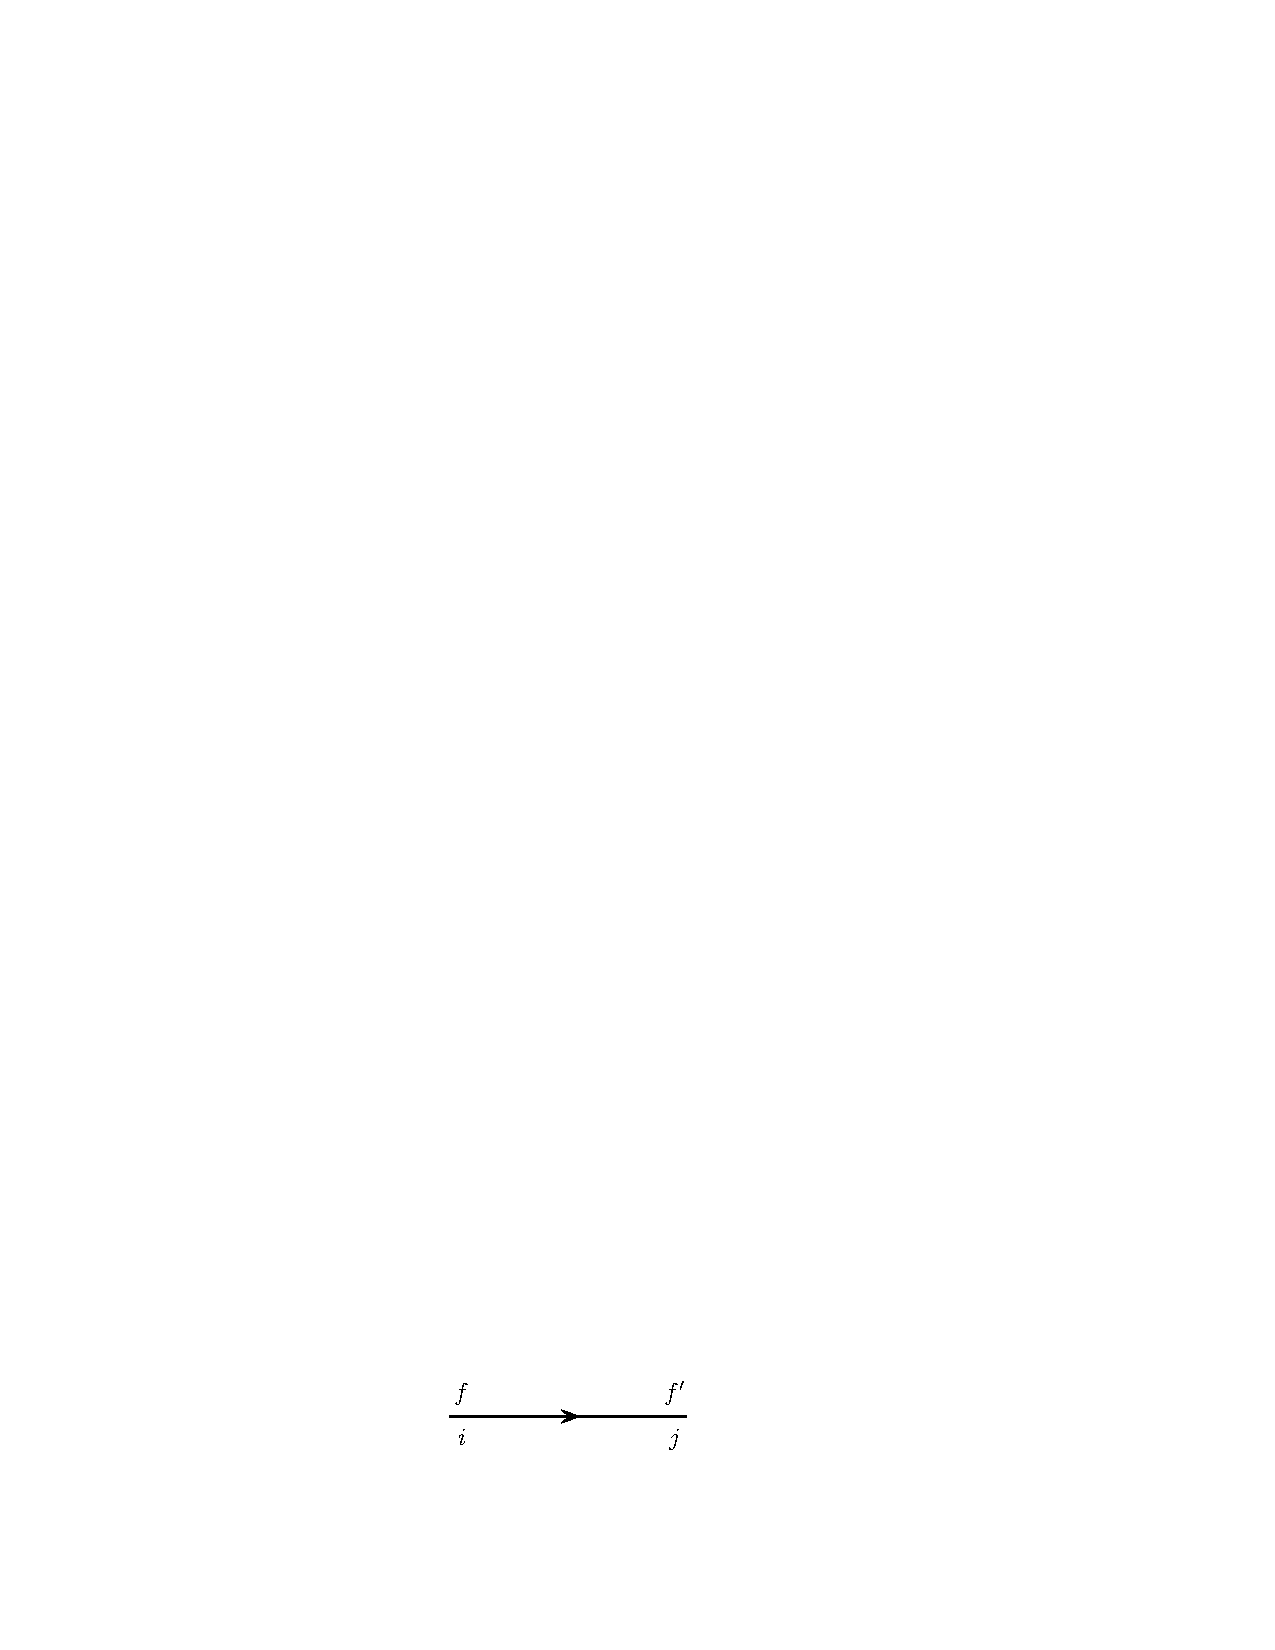
\includegraphics[width=0.5\linewidth]{quarkProp}\end{center}
				&
				\begin{center}
					\begin{equation*}
						\frac{i\delta_i^j\delta_f^{f'}(\slashed k + m)}{k^2 - m^2}
					\end{equation*}
				\end{center} \\
			% \hline
				\begin{center}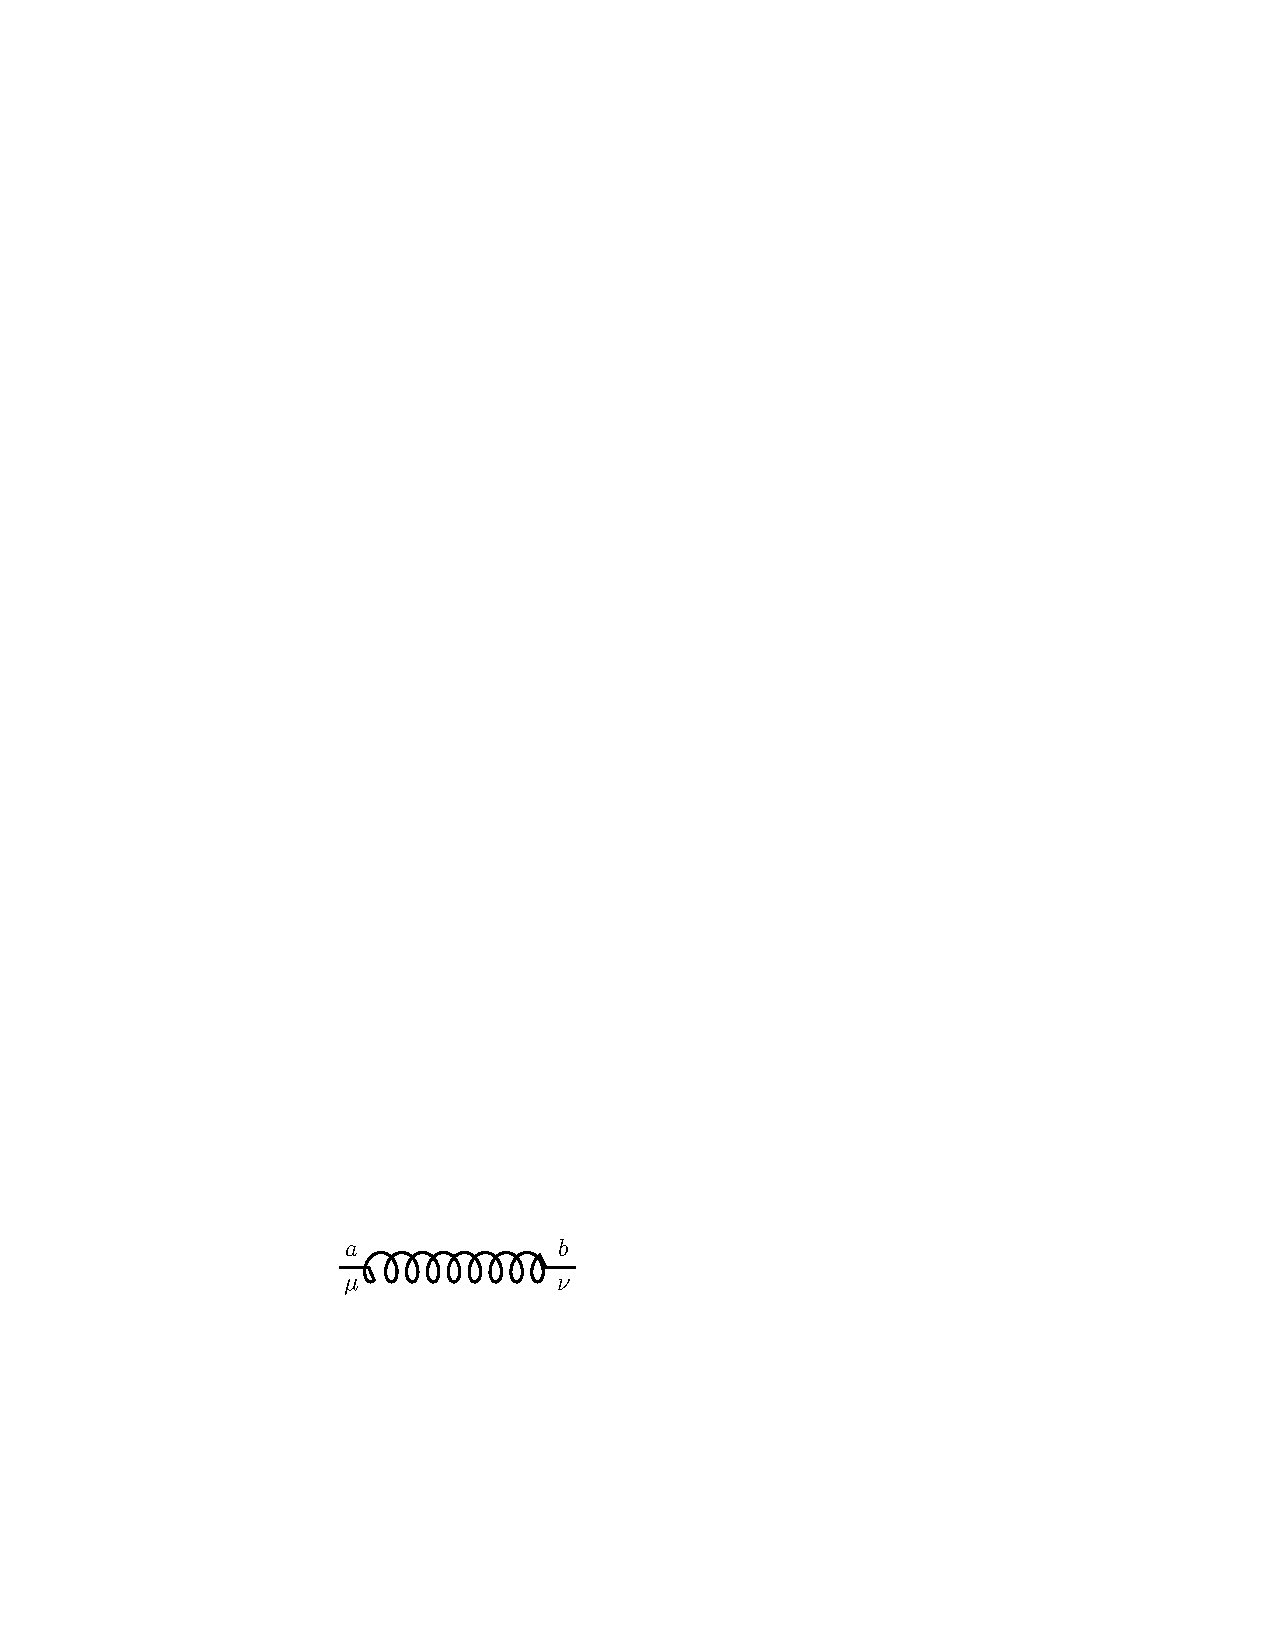
\includegraphics[width=0.5\linewidth]{gluonProp}\end{center}
				&
				\begin{center}
					\begin{equation*}
						-\frac{i\delta_a^b}{k^2}\left(g^{\mu\nu} - (\xi - 1)\frac{k^\mu k^\nu}{k^2}\right)
					\end{equation*}
				\end{center} \\
			% \hline
				\begin{center}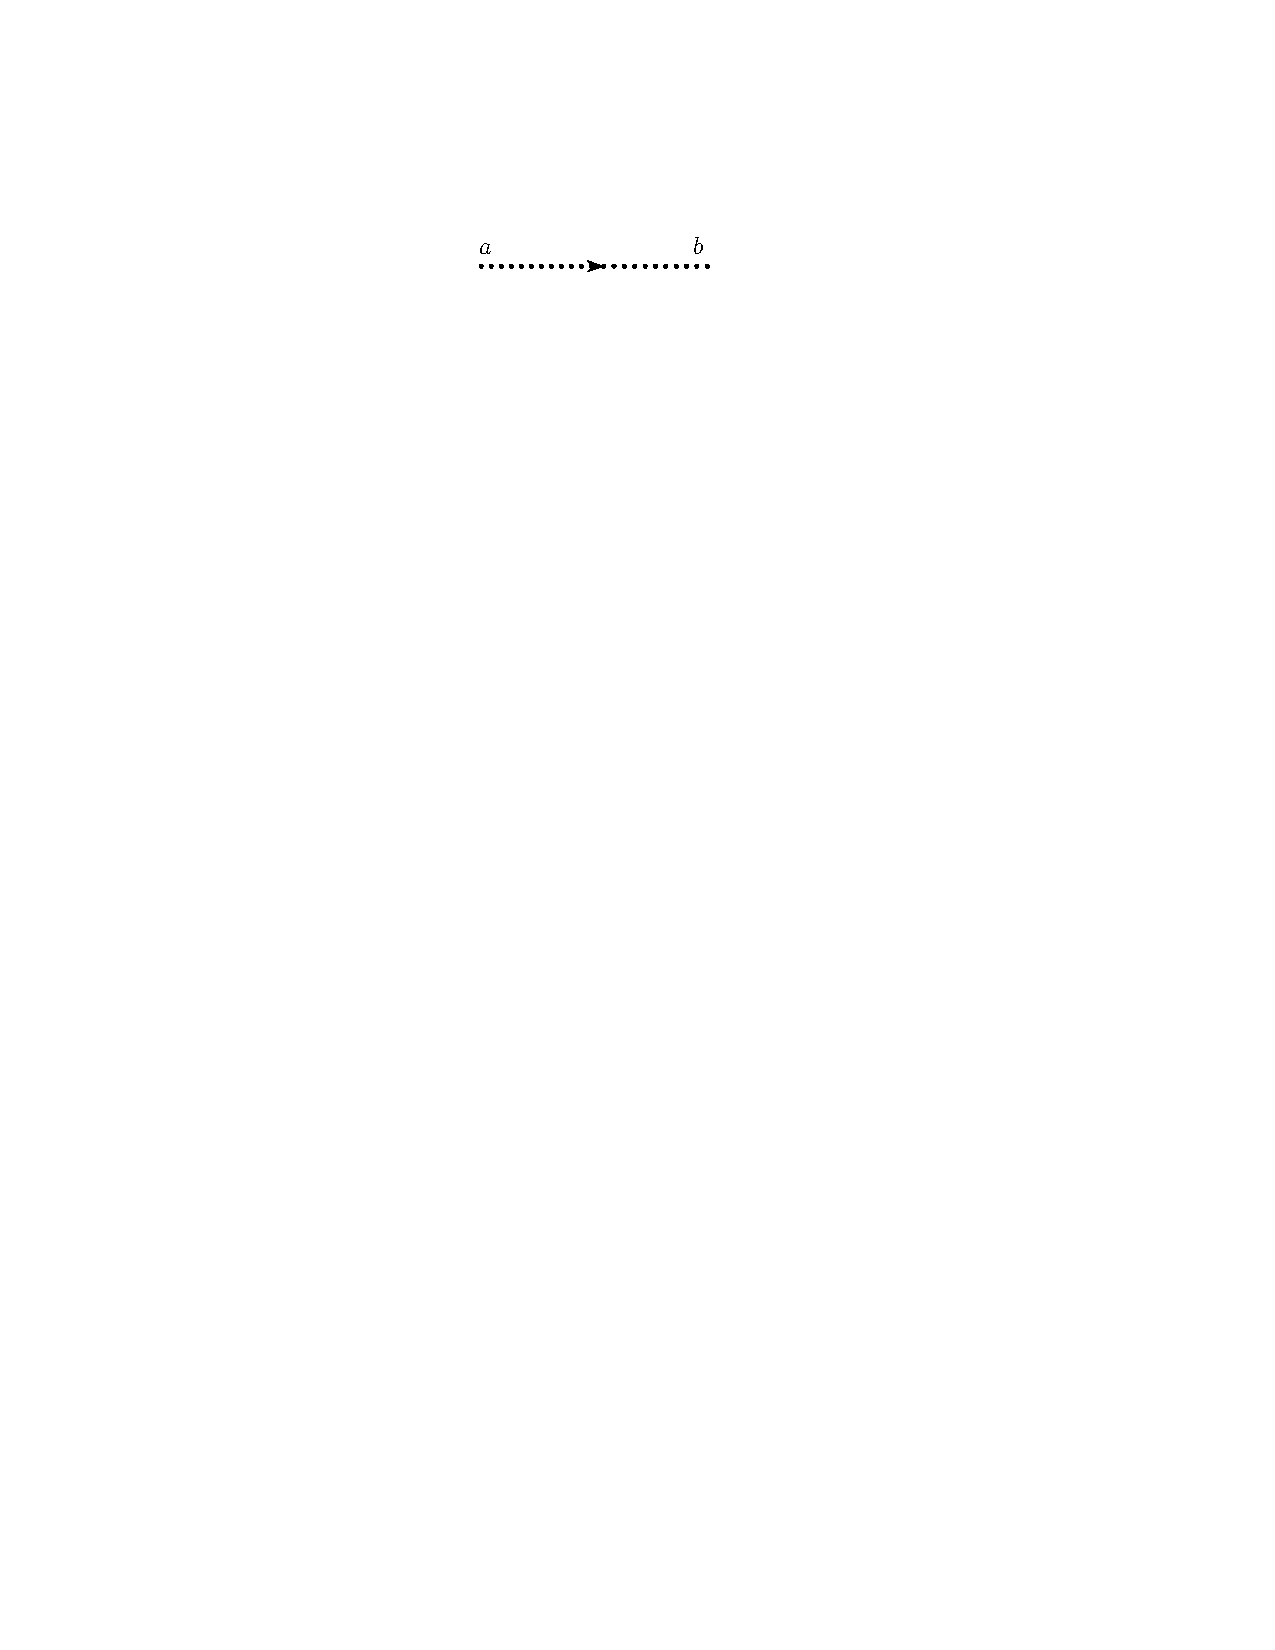
\includegraphics[width=0.5\linewidth]{ghostProp}\end{center}
				&
				\begin{center}
					\begin{equation*}
						\frac{i\delta_a^b}{k^2}
					\end{equation*}
				\end{center} \\
			% \hline
				\begin{center}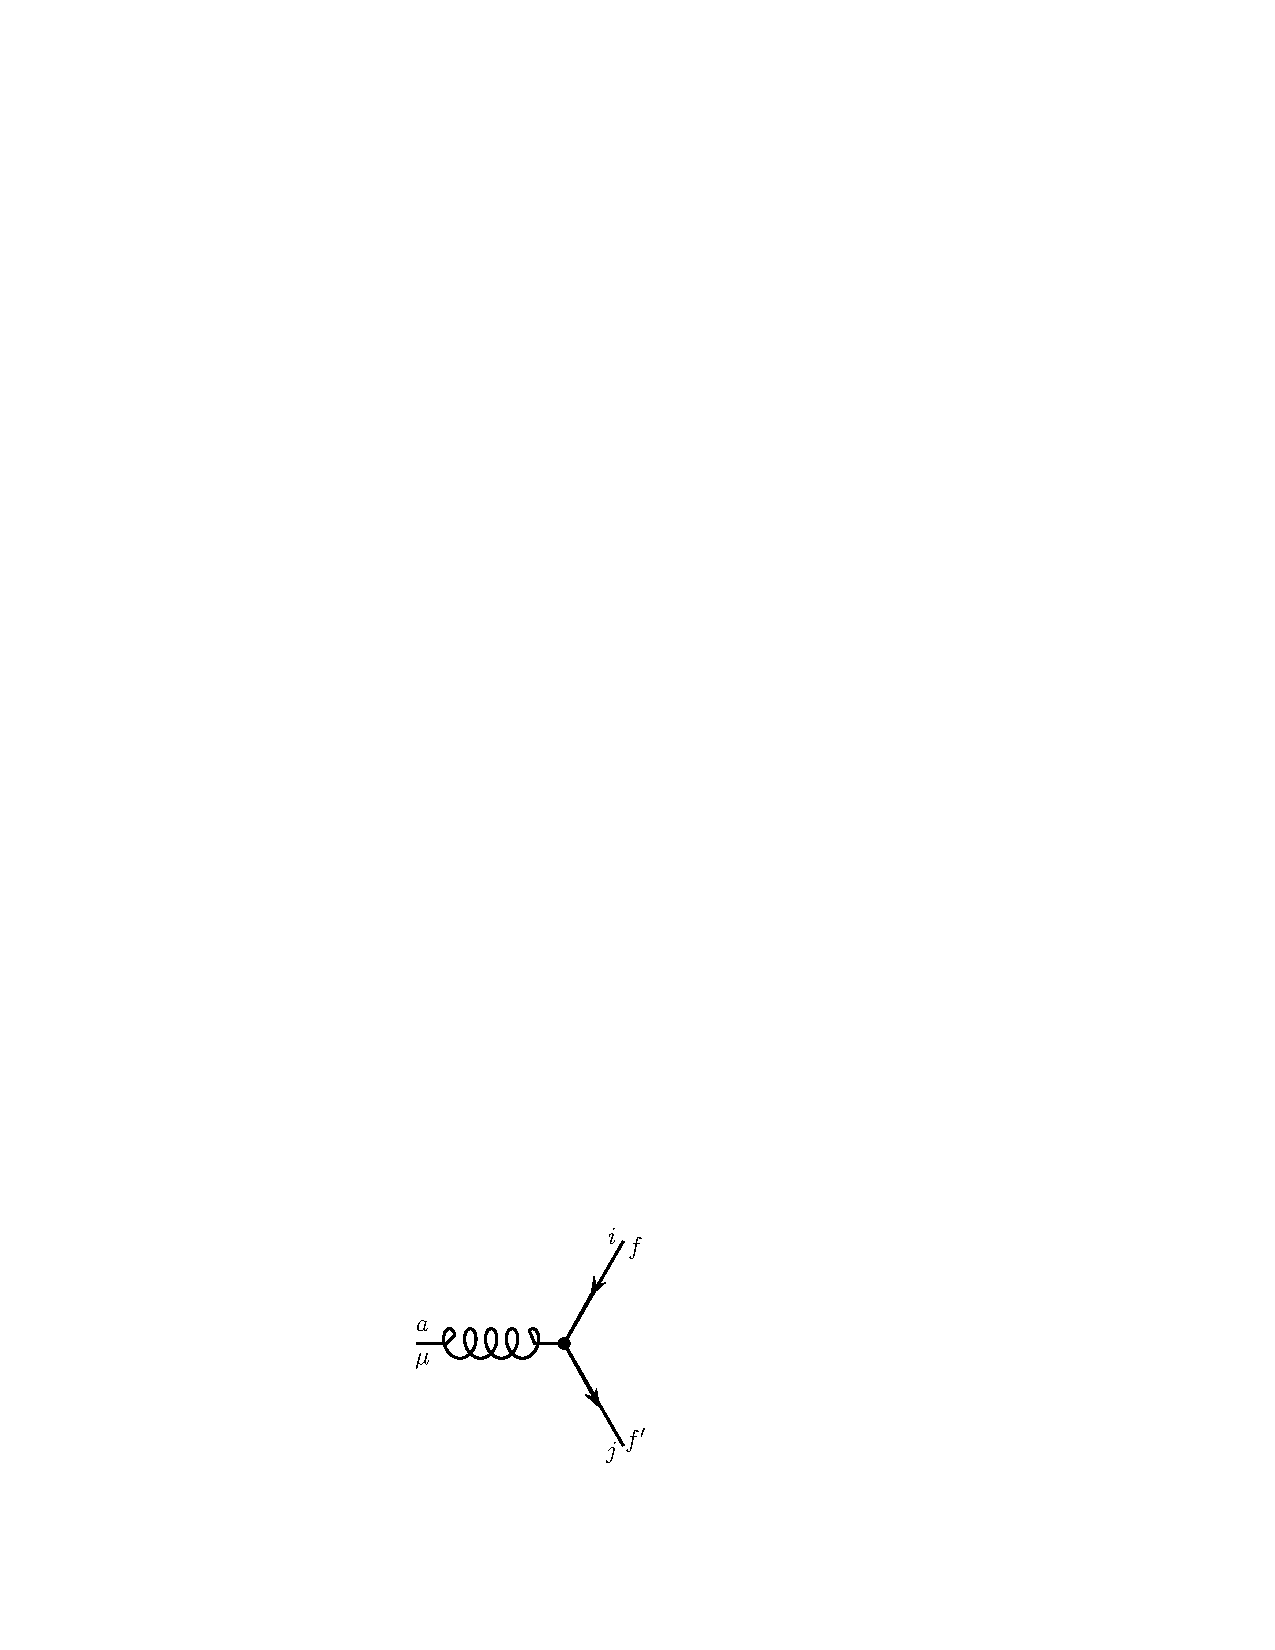
\includegraphics[width=0.40\linewidth]{qgVertex}\end{center}
				&
				\begin{center}
					\begin{equation*}
						-ig_s\gu{\mu}\delta_f^{f'}T^a_{ij}
					\end{equation*}
				\end{center} \\
			% \hline
				\begin{center}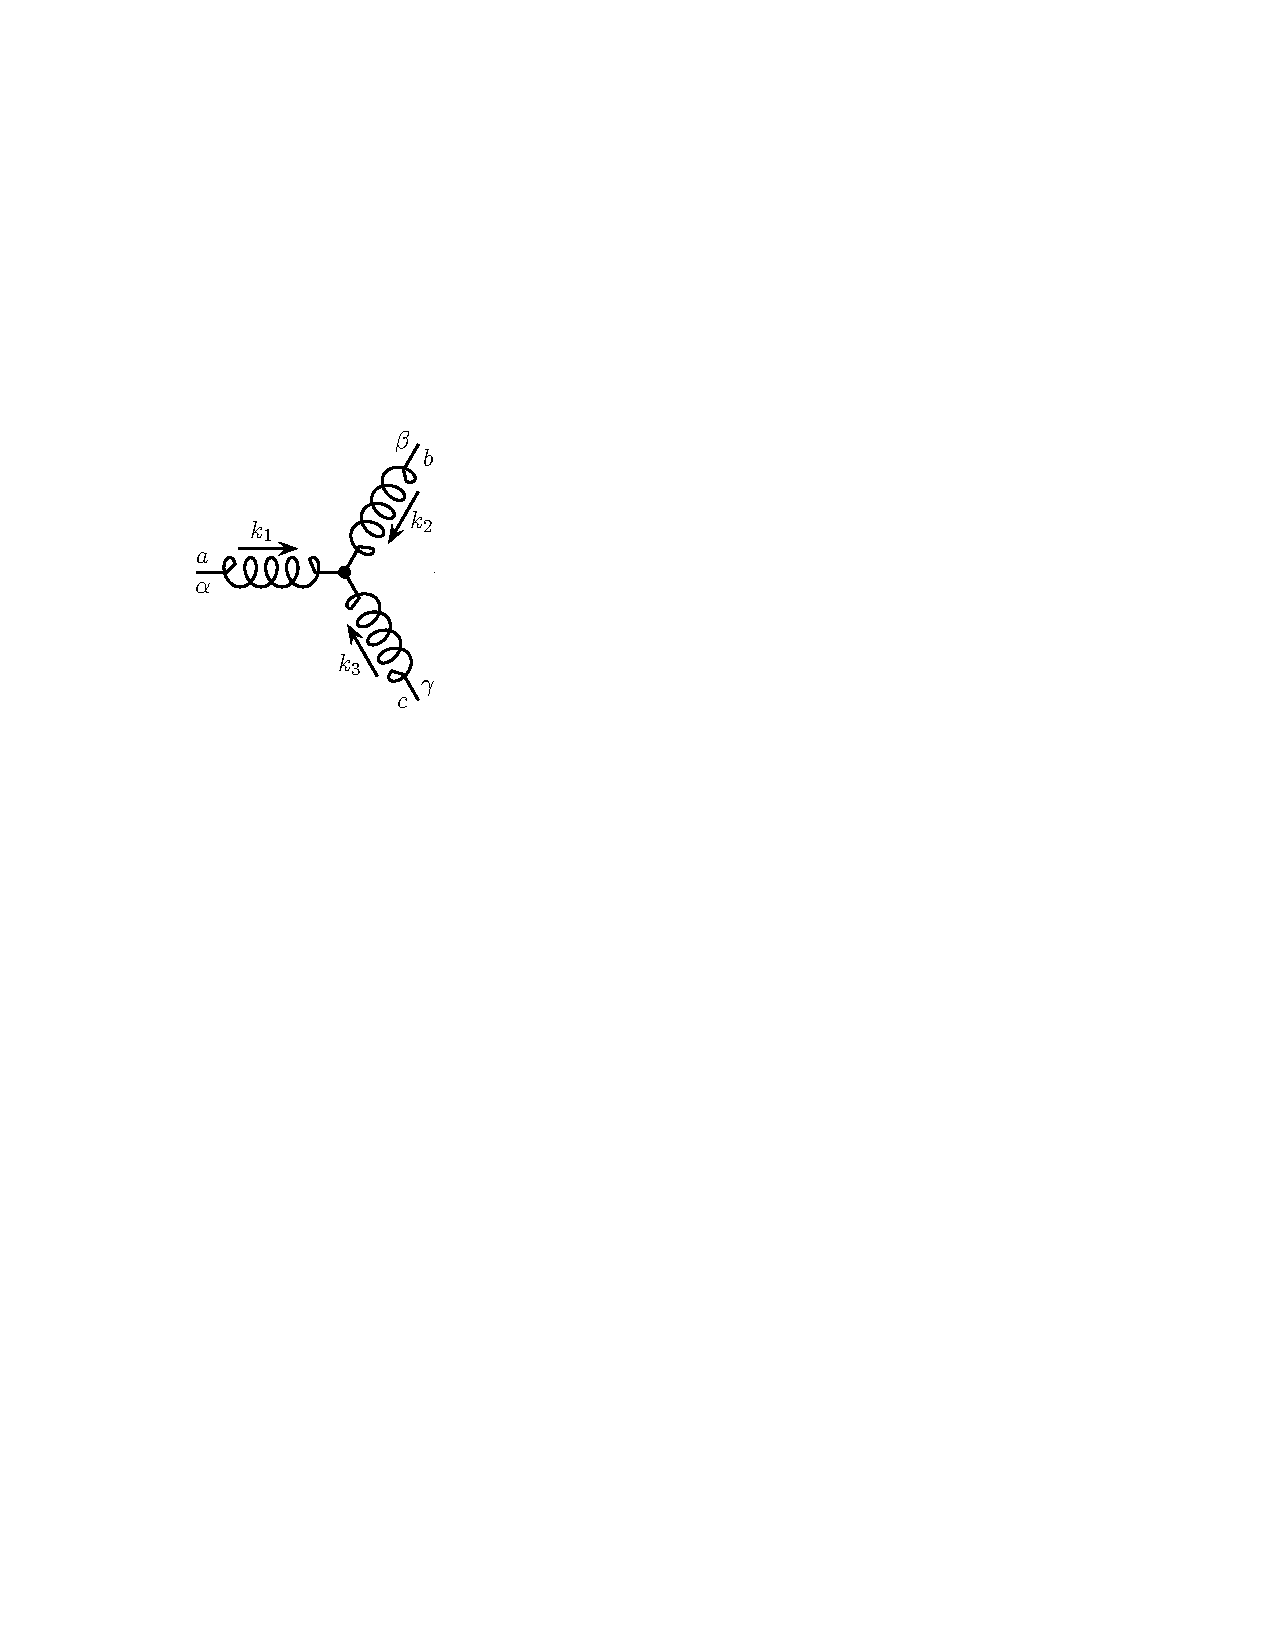
\includegraphics[width=0.40\linewidth]{tripleGluon}\end{center}
				&
				\begin{center}
					\begin{align*}
						-g_s f^{abc}\Big (g^{\alpha\beta}(k_{1} - k_{2})^{\gamma} + \\
						                  g^{\beta\gamma}(k_{2} - k_{3})^{\alpha} + \\
						                  g^{\gamma\alpha}(k_{3} - k_{1})^{\beta}\Big)
					\end{align*}
				\end{center} \\
			% \hline
				\begin{center}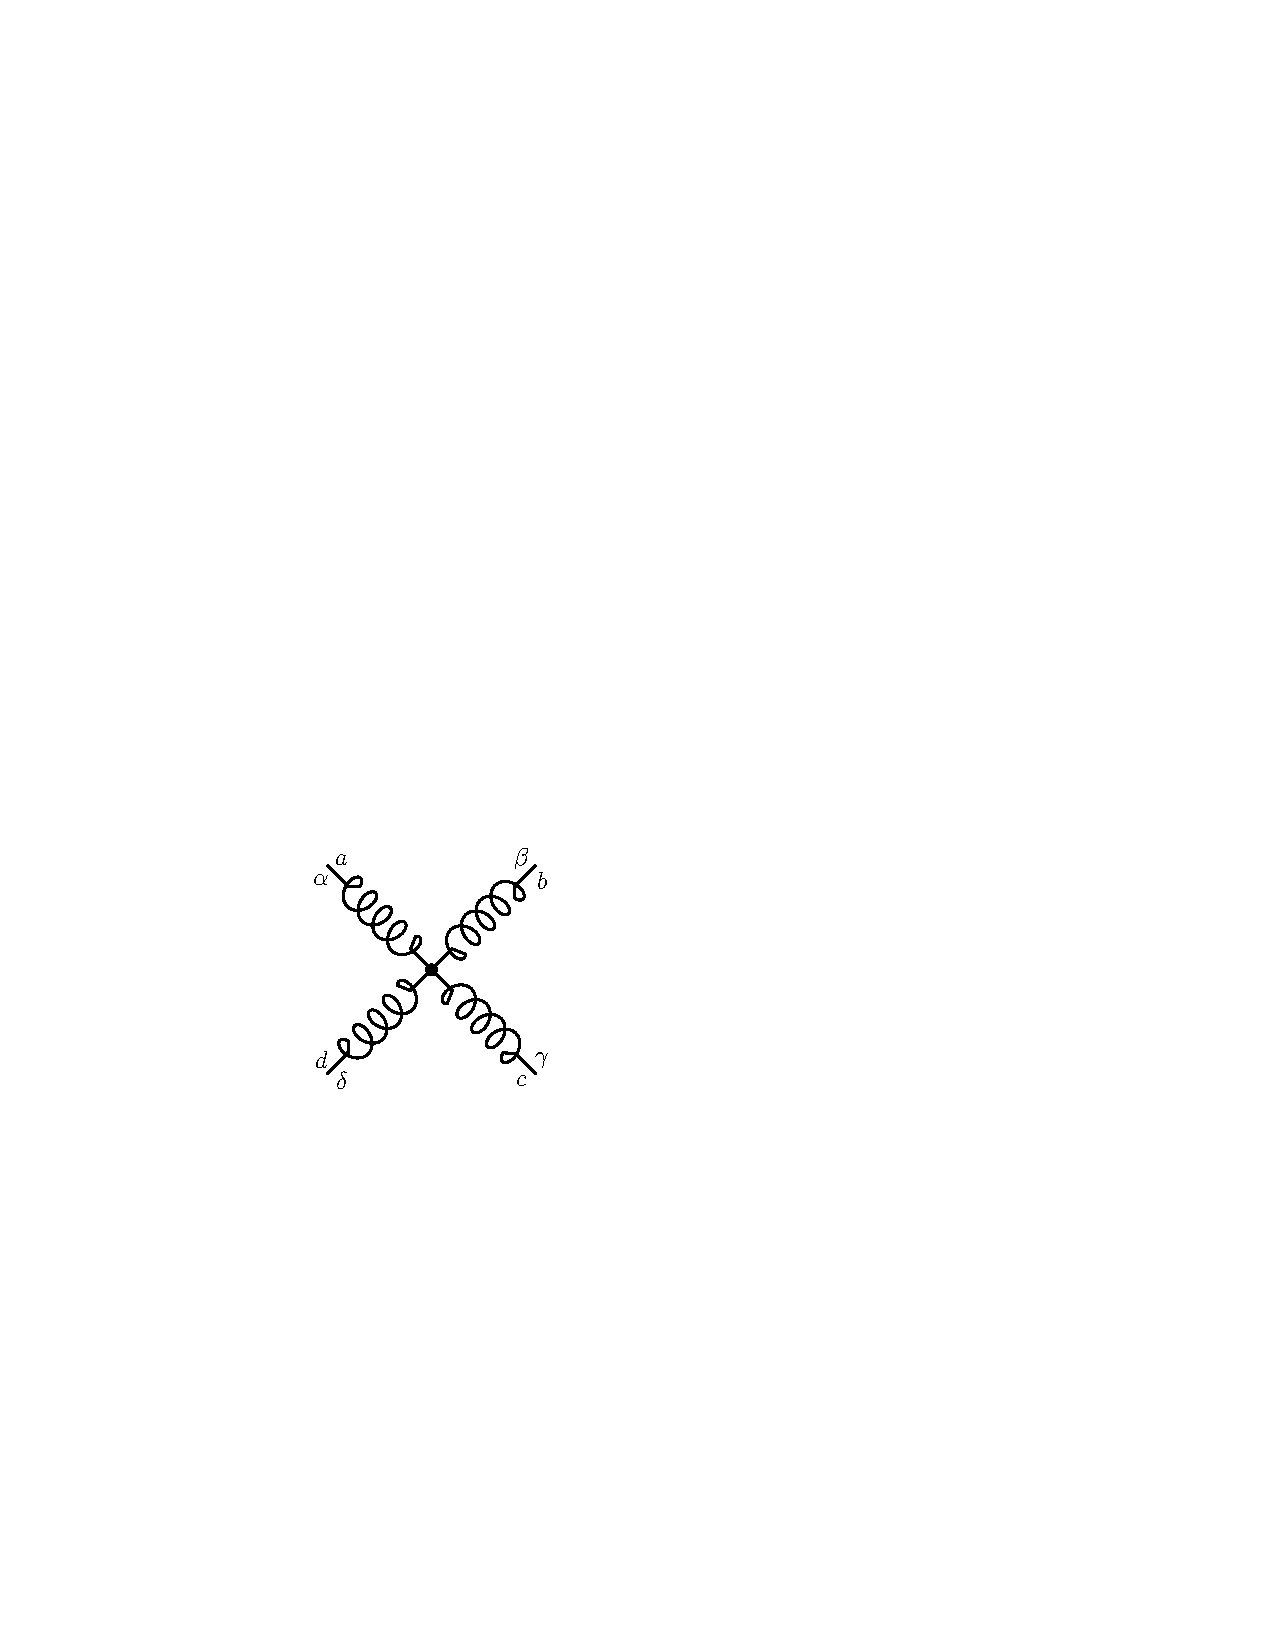
\includegraphics[width=0.40\linewidth]{quadGluon}\end{center}
				&
				\begin{center}
					\begin{align*}
						-ig_s^2\Big(f^{abe}f^{cde}(g^{\alpha\gamma}g^{\beta\delta} - g^{\alpha\delta}g^{\beta\gamma}) \\
						            f^{ace}f^{bde}(g^{\alpha\beta}g^{\gamma\delta} - g^{\alpha\delta}g^{\gamma\beta})  \\
						            f^{ade}f^{bce}(g^{\alpha\beta}g^{\delta\gamma} - g^{\alpha\gamma}g^{\delta\beta})\Big) \\
					\end{align*}
				\end{center} \\
			% \hline
				\begin{center}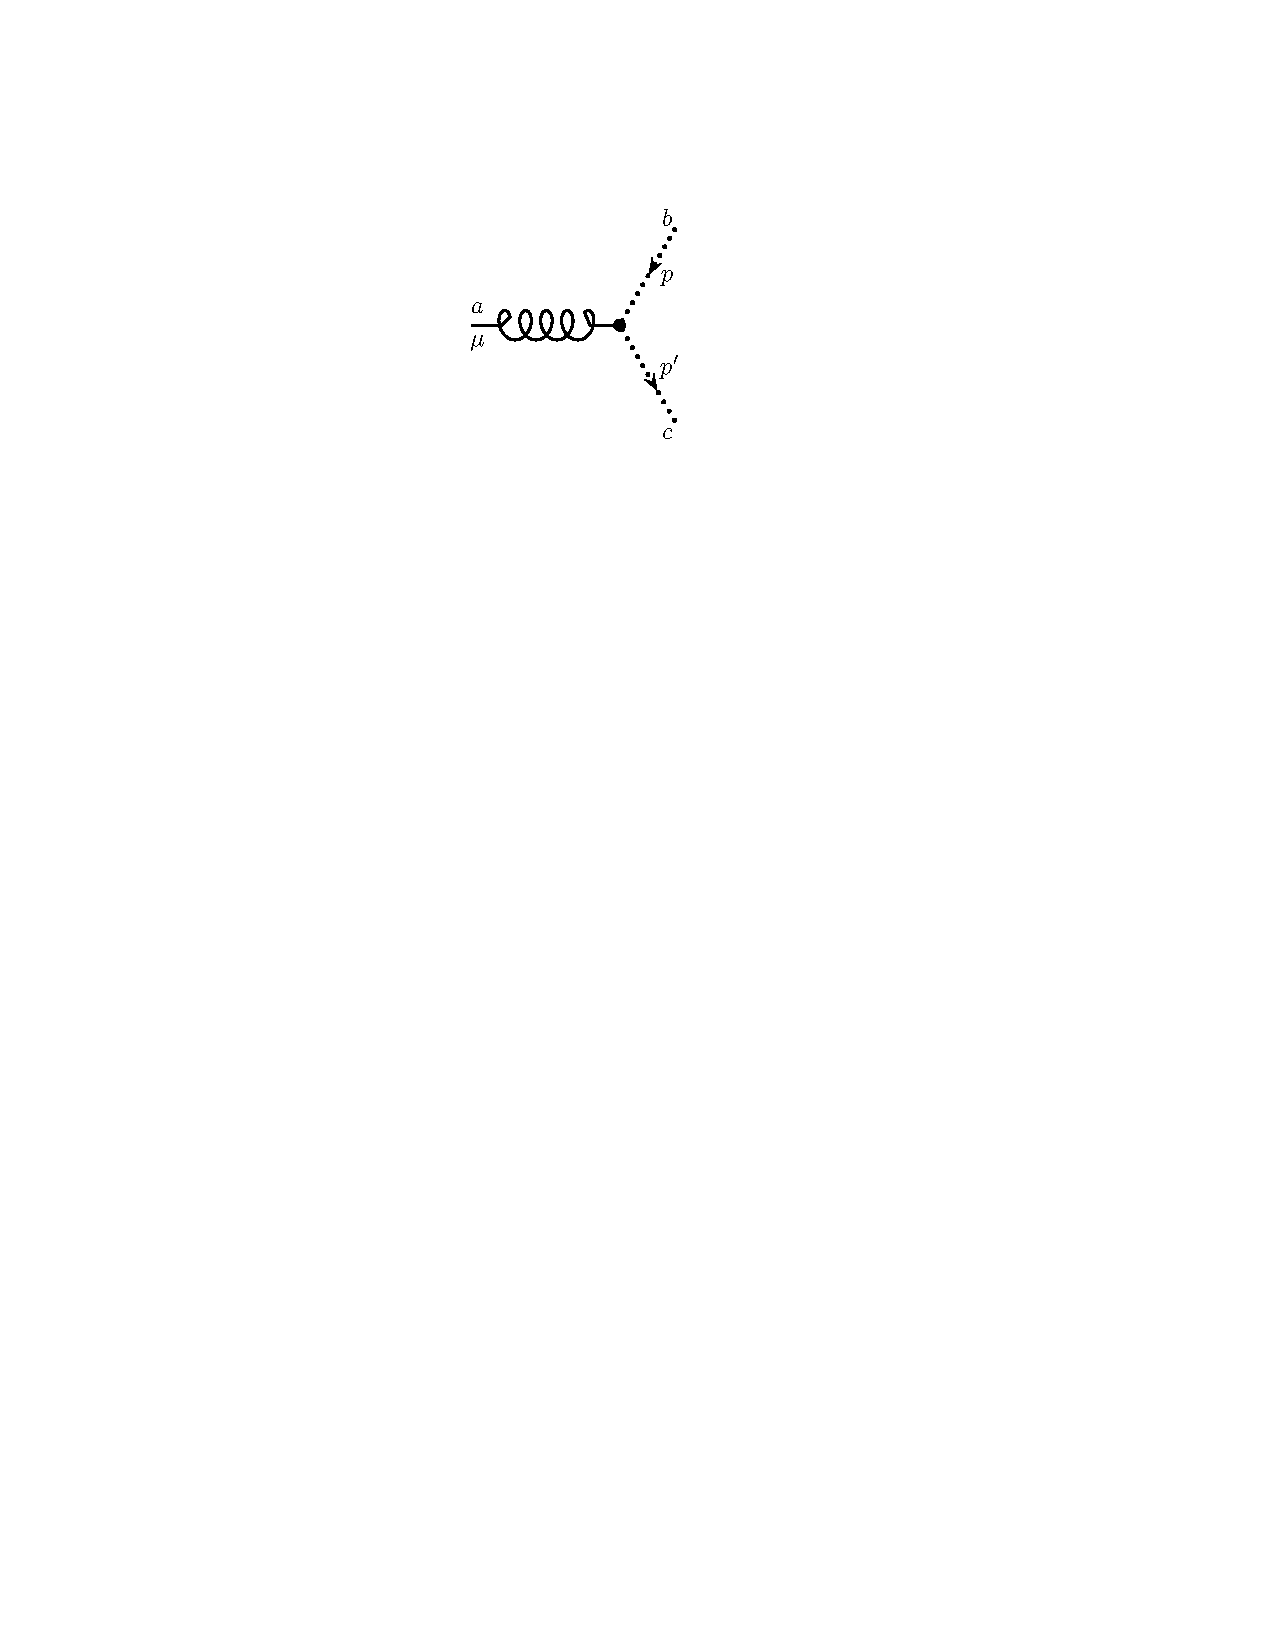
\includegraphics[width=0.40\linewidth]{gluonGhost}\end{center}
				&
				\begin{center}
					\begin{equation*}
						if^{abc}p'_{\mu}
					\end{equation*}
				\end{center} \\
			\hline
		\end{tabular}
		\label{tab:feynRules}
	\end{table}

	The first step towards this is the Lehman-Symanzik-Zimmerman (LSZ) reduction formula.  This gives us a relation between the probability
	of scattering from some initial state in to some final state, $\langle f|i\rangle\equiv\langle f|S|i\rangle$ (where $S$ is the
	scattering matrix), and a time-ordered vacuum expectation operator of a product of fields.  Here we briefly present the argument for
	the case of $2\rightarrow2$ scattering in scalar phi-cubed theory for simplicity but this generalises to more complex theories.
	The Lagrangian for this theory is given by:

	\begin{equation}
		\mathcal{L}_{\text{phi-cubed}} = \frac{1}{2}\partial^{\mu}\phi\partial_{\mu}\phi + \frac{m^2}{2}\phi^2 - \frac{g}{6}\phi^3,
		\label{eqn:phi3}
	\end{equation}

	% Firstly we must find the equation of motion for this scalar field and, upon using
	% the relativistic Euler-Lagrange equation we find $(\partial^2 + m^2)\phi = \frac{g}{2}\phi^2$.
	We can Fourier expand the field, $\phi(x)$, in terms of its annihilation and creating operators as follows:

	\begin{equation}
		\phi(x) = \int\frac{d^4k}{2E(2\pi)^3}\left(a(\vec{k})e^{ik\cdot x} + a^\dagger(\vec{k})e^{-ik\cdot x}\right).
	\end{equation}

	Inverting this we find the following form for the creating operator $a^\dagger(\vec{k})$:

	\begin{equation}
		a^\dagger(\vec{k}) = i\int d^3xe^{-ix\cdot k} \overleftrightarrow{\partial_\mu}\phi(x),
		\label{eqn:creation}
	\end{equation}

	where $f\overleftrightarrow{\partial_\mu} g = f(\partial_\mu g) - g(\partial_\mu f)$.  We expect that as time flows forward to
	$+\infty$ (or backwards to -$\infty$) the field, $\phi(x)$, become asymptotically free and therefore we can neglect and
	interaction effects in these extremes.  From equation \eqref{eqn:creation} it is straightforward to show that:

	\begin{equation}
		a^\dagger(\vec{k}, t=-\infty) - a^\dagger(\vec{k}, t=\infty) = - i\int d^4x e^{-ix\cdot k}(\partial^2 + m^2)\phi(x).
	\end{equation}

	Clearly this would be zero if we only considering the free theory where $g=0$ in equation \eqref{eqn:phi3}.  This is intuitively correct
	since once we remove any interaction terms a state we create at $t=-\infty$ should flow to $t=\infty$ unaltered.

	\subsection{Renormalising the QCD Lagrangian}

	Similarly to QED we anticipate divergent quantities in our calculations above tree level and
	so we introduce counter terms into our Lagrangian.  Similarly to equation (4) we have the following relations:

	\begin{subequations}
		\begin{equation}
			\psi_0 = Z_\psi^\frac{1}{2}\psi,
			\hspace{15mm}A_0^a = Z_A^\frac{1}{2}A^a,
			\hspace{15mm}\chi^a_0 = Z_\chi^\frac{1}{2}\chi^a,
		\end{equation}
		\begin{equation}
			m_0 = Z_mm,
			\hspace{15mm}g_{s0} = Z_sg_s,
			\hspace{15mm}\xi_0 = Z_\xi\xi.
		\end{equation}
	\end{subequations}

	Inserting these into equations (13) and (14) and rearranging so that we have
	$\mathcal{L^{QCD}} = \mathcal{L}_0 + \mathcal{L}_{ct}$ where $\mathcal{L}_0$
	is as defined in equation (13) and the counter-term Lagrangian is:

	\begin{equation}
	\begin{split}
		\mathcal{L}_{ct} = &-(Z_A - 1)\frac{1}{4}(F^a_{\mu\nu})^2 + (Z_\chi - 1)
		i(\partial^\mu\chi^a)(\partial_\mu\chi^a) + (Z_\psi - 1)\overline{\psi^i}
		(i\slashed \partial - m)\psi^i - Z_\psi(Z_m - 1)m\overline{\psi^i}\psi^i + \ldots \\
		&-(Z_sZ_A^\frac{3}{2}-1)\frac{1}{2}g_sf^{abc}\partial_{[\mu]}A^a_{\nu]}A^{b\mu}A^{c\nu} -
		(Z_s^2Z^2_A - 1)\frac{1}{4}g_s^2f^{abe}f^{cde}A^a_\mu A^b_\nu A^{c\mu}A^{d\nu} - \ldots \\
		&-(Z_sZ_\chi Z_A^\frac{1}{2} - 1)ig_sf^{abc}(\partial^\mu\chi^a)\chi^bA^c_\mu +
		(Z_sZ_\psi Z_A^\frac{1}{2} - 1)g_s\overline{\psi}^iT^a_{ij}\gamma^\mu\psi^jA^a_\mu.
	\end{split}
	\end{equation}

\section{Factorisation at Hadronic Colliders}

	\begin{itemize}
		\item Collinear factorisation which lets us pull out the PDFs as a convolution.
		\item What is a PDF? *Roughly* how are they calculated?
		\item
	\end{itemize}

\section{Divergences and Regularisation}

	\begin{itemize}
		\item How do divergences arise in QCD?  How can we deal with them?
	\end{itemize}

	In calculations above tree level we encounter divergences of various kinds which can be divided up into three classes:

	\begin{itemize}
		\item Ultraviolet (UV) divergences:  These occur when all the components of a loop momenta tend to
		infinity, $k^\alpha\rightarrow\infty$, such that $k^2$ becomes the dominant term in propagator.
		Since these extremely high momentum modes corresponding to physics at very short distance scales
		we choose to interpret these divergences as an indication that our theory is only an
		effective theory and we shouldn't attempt to apply it to all scales.

		\item Infrared (IR) divergences:  These occur in theories with massless gauge bosons, such as
		QED and QCD, since a particle may emit any number of arbitrarily such bosons with infinitesimal
		energy and we would never be able to detect their emission.  In contrast to the UV divergences
		the IR becomes important in the region of phase space where $k^2\rightarrow0$.

		\item Collinear (mass) divergences: These occur when we have massless bosons \emph{and} have
		massless on-shell particles in our calculation.  This can happen when we have, for example,
		a photon/gluon in the final state or the energy scale of the interaction is far higher than
		the mass of an emitted particle which admits taking that particles mass to be zero.
		We can see this by considering a typical propagator factor:

		\begin{equation}
			\frac{1}{(p+k)^2-m^2}\sim\frac{1}{(p+k)^2} = \frac{1}{2p\cdot k} = \frac{1}{2E_pE_k(1-\cos\theta_{pk})}.
		\end{equation}

		Where we have used the on-shell relations $p^2=0$ and $k^2=0$.  Clearly as the angle of
		emission, $\theta_{pk}$, tends to zero (the collinear limit) this term will diverge.
	\end{itemize}

	If we are to extract any useful information above tree-level we will have to find
	ways to control these infinities.  We call these methods `regularisation schemes'

	\subsection{Regularisation Schemes}

	The general plan with all regularisation schemes is to introduce a new parameter to the calculation which
	is used to get a handle on exactly \emph{how} the integral diverges.  Once we have performed the integration
	we take the limiting case where the effect of the regulator vanishes we will see that the divergence now
	presents itself as some singular function of the regulator when $\Lambda^2\rightarrow\infty$.  There are
	many ways to regularise divergences each with their own advantages and disadvantages.  We will describe a few here:

	\begin{itemize}
		\item Hard momentum cut-off: In the hard momentum cut-off approach we simply replace the upper bound
		with some finite large value, $\Lambda^2$.  This will regulate the UV and allow us to complete the
		calculation provided there are no IR or mass singularities.  While this method is very conceptually
		simple it does break both translational invariance and gauge invariance which is far from ideal.

		\item Pauli-Villars regularisation: In the Pauli-Villars scheme we replace the normal propagators with propagators damped by a large mass:

		      \begin{equation}
			      \frac{1}{p^2-m^2}\rightarrow\frac{1}{p^2-m^2} - \frac{1}{p^2-M^2}.
		      \end{equation}

		      For $m\ll M$.  Once again this does not deal with any problems with the IR/mass singularities and in order to get this
		      extra contributions we must add another field to our Lagrangian which satisfies the opposite statistics to the field we are trying to regulate.

		\item Mass regularisation: When using mass regularisation we give the gauge bosons a small mass to control any
		IR or mass divergences which might be present, we can then perform the integrals and the singularity re-emerges
		when we take the limit of massless bosons again.  The disadvantage of this scheme is that it does not regulate
		the UV region of phase space and massive gauge bosons are forbidden by gauge invariance unless we have a broken symmetry.

		\item Dimensional regularisation:  In dimensional regularisation we analytically continue the number of space-time
		dimensions away from the standard $d=4$.  We still want to be able to return to our usual 4D theory so we choose
		$d=4-2\epsilon$ where $\epsilon$ is the regulator and we plan to take the limit $\epsilon\rightarrow 0$.  The
		advantage of this is that dimensional regularisation treats both the UV and the IR divergences and both translational
		invariance and gauge invariance are preserved.  However, this modification changes the well known Dirac algebra
		relations which makes computing the numerator slightly more involved.  There are also some tensors which cannot
		easily be generalised to arbitrary dimensions.
	\end{itemize}

	\subsection{The QCD Beta function}

	\begin{itemize}
		\item How does QCD look at different scales?
		\item What is the beta function?
		\item Why is it important? How is the Beta function defined?
		\item What are the 5 diagrams needed to calculate the QCD beta function?
		\item Calculate a couple of these as an example - importance of result? Show that QCD CAN be treated perturbatively! Yaaay
	\end{itemize}

\section{Perturbative QCD and Resummation}

	\subsection{Expansions in the strong coupling constant}

	\begin{itemize}
		\item Talk about the idea of expanding the partonic cross-section etc.
	\end{itemize}

	\subsection{An Example Fixed-Order Calculation}

	\begin{figure}[tpb]
		\centering
			\begin{minipage}{0.4\linewidth}
				\centering
				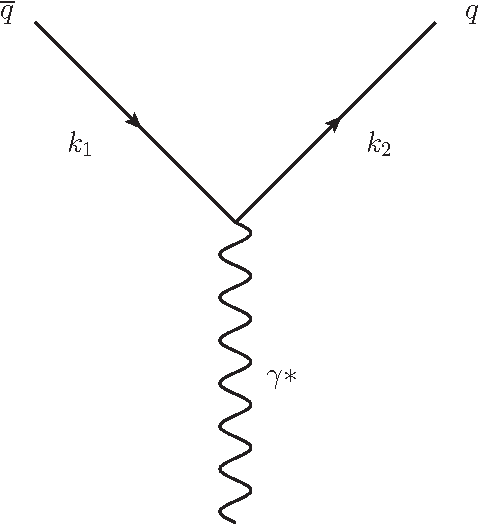
\includegraphics[width=0.98\linewidth]{TreeLevel}
				\caption{Tree level}
			\end{minipage}
			\begin{minipage}{0.4\linewidth}
				\centering
				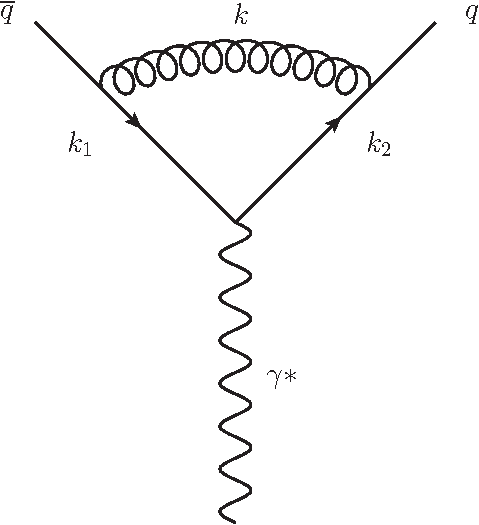
\includegraphics[width=0.98\linewidth]{NLOVirtual}
				\caption{Virtual Emission, $\mathcal{A}_v$}
			\end{minipage}
			\begin{minipage}{0.4\linewidth}
				\centering
				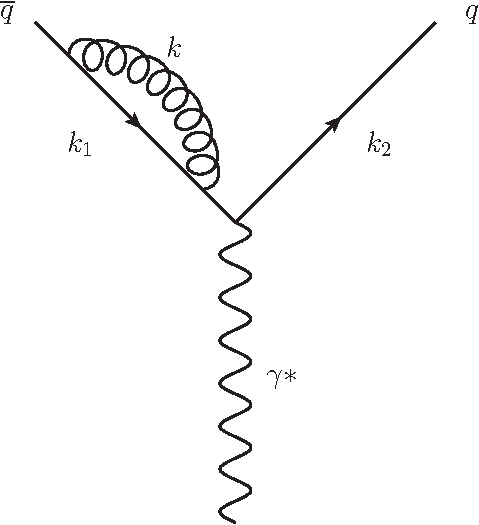
\includegraphics[width=0.98\linewidth]{NLOSelfEnergyLeft}
				\caption{Self Energy, $\mathcal{A}_{se1}$}
			\end{minipage}
			\begin{minipage}{0.4\linewidth}
				\centering
				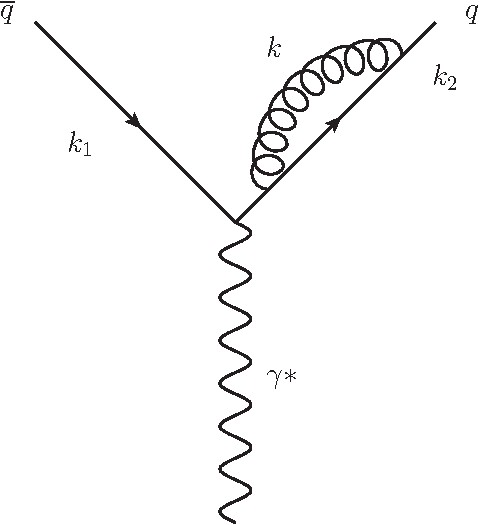
\includegraphics[width=0.98\linewidth]{NLOSelfEnergyRight}
				\caption{Self Energy, $\mathcal{A}_{se2}$}
			\end{minipage}
			\begin{minipage}{0.4\linewidth}
				\centering
				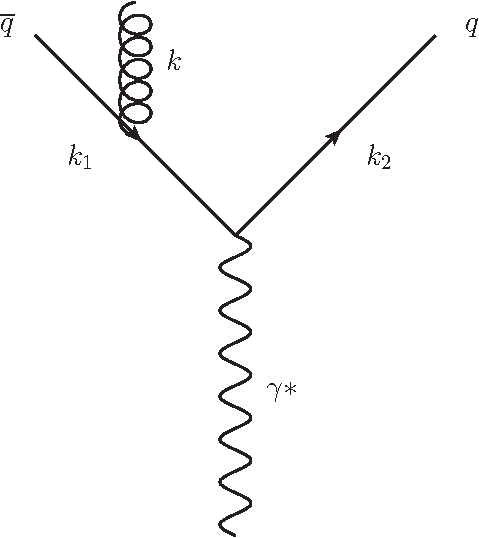
\includegraphics[width=0.98\linewidth]{NLORealLeft}
				\caption{Real Emission, $\mathcal{A}_{r1}$}
			\end{minipage}
			\begin{minipage}{0.4\linewidth}
				\centering
				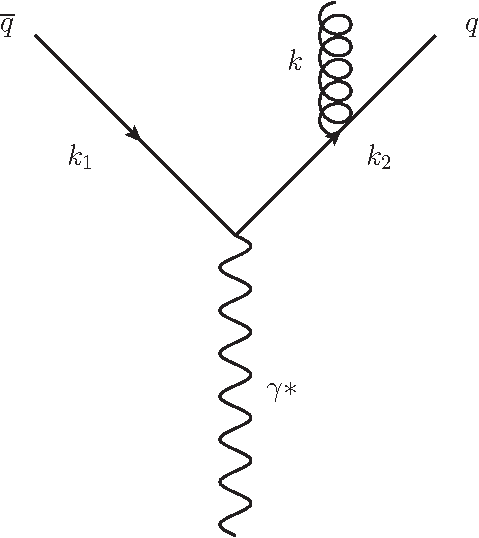
\includegraphics[width=0.98\linewidth]{NLORealRight}
				\caption{Real Emission, $\mathcal{A}_{r2}$}
			\end{minipage}
		\caption{Feynman diagrams for the $O(\alpha_s)$ correction to $\gamma^*\rightarrow q\overline{q}$
		process (a-d) and the two real emission diagrams (e-f)}\label{fig:NLOContributions}
	\end{figure}

	The Feynman diagrams which need to be included for the and $\mathcal{O}(1)$ and $\mathcal{O}(\alpha_s)$ corrections to the
	$\gamma^*\rightarrow q\overline{q}$ process are shown in figure (2).  We refer to figures (2a) as the tree level diagram,
	figure (2b) as the vertex correction and figures (2c) and (2d) as the self-energy corrections.  Figures (2e) and (2f) are
	the `real correction'.  Since the virtual corrections all have the same final state they must be summed and squared together.
	To make the order of each term in the perturbative expansion clear extract the $\alpha_s$ factors from the $\mathcal{A}_i$ here.  Therefore:

	\begin{equation}
	\begin{split}
	|\overline{\mathcal{M}}^{virtual}|^2 &= |\mathcal{A}_0 + \alpha_s\mathcal{A}_v + \alpha_s\mathcal{A}_{se1} + \alpha_s\mathcal{A}_{se2}|^2 + \mathcal{O}(\alpha_s^2) \\
	&= |\mathcal{A}_0|^2 + 2\alpha_s\Re\{\mathcal{A}^*_0\mathcal{A}_v\} + 2\alpha_s\Re\{\mathcal{A}^*_0\mathcal{A}_{se1}\} + 2\alpha_s\Re\{\mathcal{A}^*_0\mathcal{A}_{se2}\} + \mathcal{O}(\alpha_s^2).
	\end{split}
	\end{equation}

	Where the bar on the LHS means there is an implicit sum over spins and polarisations on the RHS.  We can see then that to
	$\mathcal{O}(\alpha_s)$ we have four contributions to consider, but the two self-energy contributions will have the same
	functional form so in would seem that practise we only need to perform three calculations - it turns out this is not the case;
	We will find that the divergence associated with exchanging a soft gluon in figure (2b) can only be cancelled if we also
	include the soft divergences that arise figures (2e) to (2f).  At first glance this seems very peculiar since these diagrams
	have different final states and therefore should have no business contributing to this calculation.  However, since the gluon
	can be emitted with vanishingly small momentum it would be experimentally impossible to detect and therefore the final states
	would look the same to an imperfect observer.\\It is the cancellation of these divergences that will be shown in detail
	in the next two sections.  Figures (2a), (2b) and (2e) will be calculated in detail while the result for the self energy
	expressions will only be omitted since it can be cancelled by a particular choice of gauge ~\cite{field}.  Since we
	expect both UV and IR divergences we choose to work in the dimensional regularisation scheme.

	\subsubsection{The Leading Order Process}

	If we let the pair-produced quarks have charge $Qe$ then the Feynman rules outlined in sections 2 \& 3 give:

	\begin{equation}
	\mathcal{A}_0 = -ieQ\overline{u}^{\lambda_2}(k_2)\gamma^\mu v^{\lambda_1}(k_1)\epsilon^r_\mu(p).
	\end{equation}

	Where the $\lambda_i$'s are the spins of the quarks, $r$ is the polarisation of the incoming photon and $p = k_1 + k_2$ is
	the momentum carried by the incoming photon.  To calculate we can square and since we are typically interested in unpolarised
	calculations we perform a sum over all polarisations and spins (we also choose this point to include the sum over the possible
	colour states of the outgoing quarks):

	\begin{equation}
	|\overline{\mathcal{A}_0}|^2 = 3\sum_{\forall\lambda, r}e^2Q^2[\overline{u}^{\lambda_2}(k_2)\gamma^\mu
	v^{\lambda_1}(k_1)][\overline{v}^{\lambda_1}(k_1)\gamma^\nu v^{\lambda_2}(k_1)]\epsilon^r_\mu(p)\epsilon^r_{*\mu}(p).
	\end{equation}

	We can now using Casimir's trick ~\cite{griff} to convert this spinor string into a trace, using the replacements
	$\sum_r\epsilon^r_\mu\epsilon^r_{*\nu}=-g_{\mu\nu}$ and the completeness conditions for spinors:

	\begin{equation}
	|\overline{\mathcal{A}_0}|^2 = - e^2Q^2\Tr[\slashed k_2\gamma^\mu\slashed k_1\gamma_\mu].
	\end{equation}

	Where we have used the high energy limit to discard the quark mass terms.  This trace can be evaluated in arbitrary
	dimensions to give, in the high energy limit:

	\begin{equation}
	|\overline{\mathcal{A}_0}|^2 = 6e_d^2Q^2s(d-2).
	\end{equation}

	Where we have defined the usual Mandeltam variable $s=(k_1+k_2)^2=2k_1\cdot k_2$ and defined $e_d^2=e^2\mu^{4-d}$ where
	$\mu$ has units of mass to make the coupling $e$ dimensionless.  To find the leading order cross-section we divide by the
	particle flux and multiply by the two particle phase space which is given by:

	\begin{equation}
	\int d^{2d-2}R_2 = 2^{1-d}\pi^{\frac{d}{2}-1}\frac{\Gamma(\frac{d}{2}-1)}{\Gamma(d-2)}s^\frac{d-4}{2}.
	\end{equation}

	Where $R_i$ is the $i$ final state particle phase space.  Combining these factors and defining $\alpha_e=\frac{e^2}{4\pi}$:

	\begin{equation}
	\begin{split}
	\sigma_0 &= 3\cdot2^{2-d}\pi^{1-\frac{d}{2}}\frac{\Gamma(\frac{d}{2}-1)}{\Gamma(d-2)}s^\frac{d-4}{2}4\pi\alpha\mu^{d-4}Q^2s(d-2)\frac{1}{2s} \\
	&= 3\alpha Q^2\left(\frac{s}{4\pi\mu^2}\right)^{\frac{d}{2}-2}\left(\frac{d}{2}-1\right)\frac{\Gamma(\frac{d}{2}-1)}{\Gamma(d-2)}.
	\end{split}
	\end{equation}

	and finally using $x\Gamma(x)=\Gamma(x+1)$ we get:

	\begin{equation}
	\sigma_0 = 3\alpha Q^2 \frac{\Gamma(\frac{d}{2})}{\Gamma(d-2)}\left(\frac{s}{4\pi\mu^2}\right)^{\frac{d}{2}-2}.
	\end{equation}

	It is important to note that in the limit $\epsilon\rightarrow0$ the Born cross-section remains finite.

	\subsubsection{The Virtual $\mathcal{O}(\alpha_s)$ Corrections}

	The virtual correction graphs are shown in figures (2b), (2c) and (2d).  We will begin by calculating
	the second term in equation (30).  Using the Feynman rules we have:

	\small
		\begin{subequations}
		\begin{equation}
			\mathcal{A}_v = \int\frac{d^{d}k}{(2\pi)^{d}} \overline{u}^{\lambda_2}(k_2)
			(-ig_s\mu^\epsilon\gamma^\alpha T^a_{ij})\frac{i(\slashed k_1 + \slashed k)}{(k_1+k)^2}
			(-ieQ\gamma^\mu)\frac{i(\slashed k_2 - \slashed k)}{(k_2 - k)^2}(-g_s\mu^\epsilon\gamma^\beta T^a_{ij})
			\epsilon^r_\mu(p)\frac{-i}{k^2}\left(g_{\alpha\beta} +
			(1-\xi)\frac{k^\alpha k^\beta}{k^2}\right)v^{\lambda_1}(k_1).
		\end{equation}
		\begin{equation}
			\mathcal{A}_v = -ig_s^2eQ\mu^{2\epsilon}\Tr(T^aT^a)\overline{u}^{\lambda_2}
			(k_2)\int\frac{d^{d}k}{(2\pi)^{d}}\frac{\mathcal{N}_1(k_1, k_2, k)}{k^2(k_1+k)^2(k_2-k)^2}v^{\lambda_2}(k_2).
		\end{equation}
		\end{subequations}
	\normalsize

	Where the numerator of the fraction is given by:

	\begin{equation}
	\mathcal{N}_1(k_1, k_2, k) = \gamma^\alpha(\slashed k_1 + \slashed k)\gamma^\mu(\slashed k_2 -
	\slashed k)\gamma_\beta\Big(g^{\alpha\beta} + (1-\xi)\frac{k^\alpha k^\beta}{k^2}\Big).
	\end{equation}

	From equation (30) we see we need $\mathcal{A}_0^*\mathcal{A}_v$:

	\begin{equation}
		\mathcal{A}_0^*\mathcal{A}_v = g_s^2e^2Q^2\Tr(T^aT^a)[\overline{v}^{\lambda_1}(k_1)\gamma^\nu u(k_2)]
		\left[\overline{u}^{\lambda_2}(k_2)\int\frac{d^{d}k}{(2\pi)^{d}}\frac{\mathcal{N}_1(k_1, k_2, k)}
		{k^2(k_1+k)^2(k_2-k)^2}v^{\lambda_1}(k_1)\right]\epsilon^r_{\mu}(p)\epsilon^r_{*\nu}(p).
	\end{equation}

	And now performing the spin/polarisation/colour sum and average gives:

	\begin{equation}
	\overline{\mathcal{A}_0^*\mathcal{A}_v} = -\frac{g_s^2e^2Q^2}{2}\int\frac{d^{d}k}
	{(2\pi)^{d}}\frac{\mathcal{N}_2(k_1, k_2,k)}{k^2(k_1+k)^2(k_2-k)^2}.
	\end{equation}

	Where:

	\begin{equation}
	\mathcal{N}_2(k_1, k_2, k) = \Tr[\slashed k_1 \gamma_\alpha(\slashed k_1 + \slashed k)\gamma_\mu
	(\slashed k_2 - \slashed k)\gamma_\beta\slashed k_2\gamma^\mu]\Big(g^{\alpha\beta} + (1-\xi)\frac{k^\alpha k^\beta}{k^2}\Big).
	\end{equation}

	Before we can proceed any further we must evaluate the trace term in the integral.  As mentioned in section X
	this is not as easy as it seems because, although the Dirac matrices still satisfy the Clifford algebra, the
	various identities for their contractions and traces change when we are in $d$ dimensions.  Two useful examples are shown below:

	\begin{subequations}
	\begin{equation}
	g_{\mu\nu}g^{\mu\nu} = d
	\end{equation}
	\begin{equation}
	\gamma^\mu\gamma_\nu\gamma_\mu = (d-2)\gamma_nu
	\end{equation}
	\end{subequations}

	Using the \texttt{FORM} package ~\cite{form} to perform the two trace terms present gives:

	\begin{equation}
	\begin{split}
	\Tr[\slashed k_1 \gamma_\alpha(\slashed k_1 + \slashed k)\gamma_\mu(\slashed k_2 &-
	\slashed k)\gamma^\alpha\slashed k_2\gamma^\mu] = s[s(8-4d) + \frac{(k_1\cdot k)(k_2\cdot k)}{s}(32-16d) \\
	&- (16-8d)(k_1\cdot k - k_2\cdot k) + k^2(16-12d+2d^2)].
	\end{split}
	\end{equation}

	\begin{equation}
	\begin{split}
	\Tr[\slashed k_1 \gamma_\alpha(\slashed k_1 + \slashed k)\gamma_\mu(\slashed k_2 &- \slashed k)\gamma_\beta
	\slashed k_2\gamma^\mu]k^\alpha k^\beta = s[(k_1\cdot k)(k_2\cdot k)(16 - 8d) \\
	&+ k^2(8 - 4d)(k_2\cdot k - k_1\cdot k) - k^4(4 - 2d)].
	\end{split}
	\end{equation}

	Where $s = 2k_1\cdot k_2$ and we have used the on-shell relations.  After factorising the terms
	quadratic in $d$ and combining the two trace terms we arrive at:

	\begin{equation}
	\overline{\mathcal{A}_0^*\mathcal{A}_v} = -4s\left(\frac{d}{2}-1\right)\frac{g_s^2e^2Q^2}{2}
	\int\frac{d^{d}k}{(2\pi)^{d}}\frac{\mathcal{N}_3(k_1, k_2, k)}{k^2(k_1+k)^2(k_2-k)^2}.
	\end{equation}

	Where:

	\begin{equation}
	\mathcal{N}_3(k_1, k_2, k) = -2s + \frac{8k\cdot k_1k\cdot k_2}{s} + (6+2\xi)(k\cdot k_1 -
	k\cdot k_2) + k^2(d-4) - 4(1-\xi)\frac{k\cdot k_1 k\cdot k_2}{k^2} - (1-\xi)k^2.
	\end{equation}

	Combining this with the particle flux and the two particle phase space we can write an expression
	for the vertex corrected cross-section.  Once again we scale the couplings such that they remain
	dimensionless by defining $g_d^2=g_s^2\mu^{2-\frac{d}{2}}$:

	\begin{subequations}
	\begin{equation}
	\sigma_v = -4s\left(\frac{d}{2}-1\right)\frac{g_d^2\mu^{2-\frac{d}{2}}e^2Q^2}{4s}2^{1-d}\pi^{\frac{d}{2}-1}
	\frac{\Gamma(\frac{d}{2}-1)}{\Gamma(d-2)}s^\frac{d-4}{2}\int\frac{d^{d}k}{(2\pi)^{d}}\frac{\mathcal{N}_3(k_1, k_2, k)}{k^2(k_1+k)^2(k_2-k)^2},
	\end{equation}
	\begin{equation}
	\Rightarrow\sigma_v = -g_d^2\mu^{2-\frac{d}{2}}Q^2 4\pi\alpha\mu^{4-d}2^{1-d}\pi^{\frac{d}{2}-1}\frac{\Gamma(
	\frac{d}{2})}{\Gamma(d-2)}s^\frac{d-4}{2}\int\frac{d^{d}k}{(2\pi)^{d}}\frac{\mathcal{N}_3(k_1, k_2, k)}{k^2(k_1+k)^2(k_2-k)^2},
	\end{equation}
	\begin{equation}
	\Rightarrow\sigma_v = -\frac{4\sigma_0}{3}g_d^2\mu^{2-\frac{d}{2}}\int\frac{d^{d}k}{(2\pi)^{d}}
	\frac{\mathcal{N}_3(k_1, k_2, k)}{k^2(k_1+k)^2(k_2-k)^2}.
	\end{equation}
	\end{subequations}

	Where we have expressed the virtual rate as a multiplicative correction to the Born level rate
	by comparing directly with equation (35).  We must now use the Feynman parametrisation to re-express
	the product of propagators as a sum by introducing new integration variables.  Using:

	\begin{equation}
	\frac{1}{ab} = \int_0^1dy\frac{1}{(ay+b(1-y))^2}.
	\end{equation}

	We have that:

	\begin{equation}
	\sigma_v = -\frac{4\sigma_0}{3}g_d^2\mu^{2-\frac{d}{2}}\int\frac{d^{d}k}{(2\pi)^d}
	\int_0^1dy\frac{\mathcal{N}_3(k_1, k_2, k)}{(k^2-2k\cdot k_y)^2k^2}.
	\end{equation}

	Where $k_y = yk_1 -(1-y)k_2$.  Examining now the integrand we see there are two
	different $k$ dependences and so we partition the terms as follows:

	\begin{equation}
	\sigma_v = -\frac{4\sigma_0}{3}g_d^2\mu^{2-\frac{d}{2}}\int\frac{d^{d}k}{(2\pi)^d}\int_0^1dy
	\left(\frac{\mathcal{N}'_3(k_1, k_2, k)}{(k^2-2k\cdot k_y)^2k^2} +
	\frac{\mathcal{N}''_3(k_1, k_2, k)}{(k^2-2k\cdot k_y)^2k^4}\right).
	\end{equation}

	Where:

	\begin{subequations}
	\begin{equation}
	\mathcal{N}'_3(k_1, k_2, k) = -2s + \frac{8k\cdot k_1k\cdot k_2}{s} +
	(6+2\xi)(k\cdot k_1 - k\cdot k_2) + k^2(d-4) - (1-\xi)k^2.
	\end{equation}
	\begin{equation}
	\mathcal{N}''_3(k_1, k_2, k) = - 4(1-\xi)k\cdot k_1 k\cdot k_2.
	\end{equation}
	\end{subequations}

	Differentiating equation with respect to $c$ and $d$ (47) we get the following useful parametrisations:

	\begin{subequations}
	\begin{equation}
	\frac{1}{c^2d} = \int_0^1dx\frac{2x}{(cx+d(1-x))^3},
	\end{equation}
	\begin{equation}
	\frac{1}{c^2d^2} = \int_0^1dx\frac{6x(1-x)}{(cx+d(1-x))^4}.
	\end{equation}
	\end{subequations}

	and taking $c = k^2-2k\cdot k_y$ and $d = k^2$, simplifying the denominators and performing a change of variables $K=k-xp_y$ yields:

	\begin{equation}
	\sigma_v = -\frac{4\sigma_0}{3}g_d^2\mu^{2-\frac{d}{2}}\int\frac{d^{d}K}{(2\pi)^d}\int_0^1dy\int_0^1dx
	\left(\frac{2x\mathcal{N}'_3(k_1, k_2, K+xk_y)}{(K^2-C)^3} + \frac{6x(1-x)
	\mathcal{N}''_3(k_1, k_2, K+xk_y)}{(K^2-C)^4}\right).
	\end{equation}

	Where $C = x^2p_y^2$.  The change of variables modifies the numerator terms to:

	\begin{subequations}
	\begin{equation}
	\mathcal{N}'_3(k_1, k_2, K+xk_y) = -2s + K^2\left(\frac{4}{d} + d - 5 + \xi\right) - (3 + \xi)xs + x^2ys(1-y)(3-d-\xi),
	\end{equation}\begin{equation}
	\mathcal{N}''_3(k_1, k_2, K+xk_y) = (1-\xi)\left(x^2ys^2(1-y)-\frac{2s}{d}K^2\right).
	\end{equation}
	\end{subequations}

	We can now perform the integrations over $K$ with the aid of equation (54):

	\begin{equation}
	\int\frac{d^{d}K}{(2\pi)^d}\frac{(K^2)^m}{(K^2-C)^n} = \frac{i(-1)^{m-n}}{(4\pi)^\frac{d}{2}}
	C^{m-n+\frac{d}{2}}\frac{\Gamma(m+\frac{d}{2})\Gamma(n-m-\frac{d}{2})}{\Gamma(\frac{d}{2})\Gamma(n)}.
	\end{equation}

	Looking at the $K$ structure of equation (53) we can see that there are going to be 4 forms
	of equation (54) needed in this calculation.  I will not show the calculation for every integral
	but will show one as an example of how the calculations can proceed.  Consider the contribution of the first term of (53a):

	\begin{equation}
	-4s\int_0^1dy\int_0^1dxx\int\frac{d^{d}K}{(2\pi)^d}\frac{1}{(K^2-C)^3} = 4si\int_0^1dy\int_0^1dxx(4\pi)^{-\frac{d}{2}}
	C^{-3+\frac{d}{2}}\frac{\Gamma(\frac{d}{2})\Gamma(3-\frac{d}{2})}{\Gamma(\frac{d}{2})\Gamma(3)}.
	\end{equation}

	From above we see that $C=x^2k_y=-x^2y(1-y)s$ and so:

	\begin{equation}
	\Rightarrow=4si(4\pi)^{-\frac{d}{2}}\Gamma(3-\frac{d}{2})(-s)^{-3+\frac{d}{2}}\int_0^1dy\int_0^1dxx^{-5+d}
	y^{\left(-2+\frac{d}{2}\right)-1}(1-y)^{\left(-2+\frac{d}{2}\right)-1}.
	\end{equation}

	Where we have written the $y$ exponents in such a way that we can use the following ~\cite{field}:

	\begin{equation}
	\int_0^1dxx^{a-1}(1-x)^{b-1}=\frac{\Gamma(a)\Gamma(b)}{\Gamma(a+b)}.
	\end{equation}

	Therefore:

	\begin{equation}
	\Rightarrow=4si(4\pi)^{-\frac{d}{2}}\Gamma\left(3-\frac{d}{2}\right)(-s)^{-3+\frac{d}{2}}
	\frac{1}{d-4}\frac{\Gamma^2(\frac{d}{2}-2)}{\Gamma(d-4)}.
	\end{equation}

	Which, after choosing $d=4+\epsilon$ (with the intention of taking the limit $\epsilon\rightarrow0$
	once it is safe to do so), and manipulating the gamma functions to expose the pole structure gives:

	\begin{equation}
	-4\int_0^1dy\int_0^1dxx\int\frac{d^{d}K}{(2\pi)^d}\frac{1}{(K^2-C)^3} = 4(-s)^{\frac{\epsilon}{2}}i(4\pi)^{-2-\frac{\epsilon}{2}}
	\frac{4}{\epsilon^2}\frac{\Gamma\left(1-\frac{\epsilon}{2}\right)\Gamma^2\left(1+\frac{\epsilon}{2}\right)}{\Gamma(1+\epsilon)}.
	\end{equation}

	Which is clearly divergent in the limit $d\rightarrow4$.  The other integrals follow similarly and
	the combined result (simplified with the aid of a computer package) can be expressed as:

	\begin{equation}
	\sigma_v = \frac{2\alpha_s}{3\pi}\sigma_0\Big(\frac{s}{4\pi\mu^2}\Big)^{\frac{\epsilon}{2}}\frac{\Gamma
	\Big(1-\frac{\epsilon}{2}\Big)\Gamma^2\Big(1+\frac{\epsilon}{2}\Big)}{\Gamma(1+\epsilon)}\Big(-\frac{8}{\epsilon^2} +
	\frac{6}{\epsilon} - \frac{8+4\epsilon}{1+\epsilon}\Big).
	\end{equation}

	Where we have defined $\alpha_s=\frac{g_d^2}{4\pi}$ and using \texttt{Maple} to expand the
	product of gamma matrices for $\epsilon\rightarrow0$ gives:

	\begin{subequations}
	\begin{equation}
	\frac{\Gamma\left(1-\frac{\epsilon}{2}\right)\Gamma^2\left(1+\frac{\epsilon}{2}\right)}{\Gamma(1+\epsilon)} =
	\frac{\gamma_E}{2}\epsilon + \left(\frac{\gamma_E^2}{8} - \frac{\pi^2}{48}\right)\epsilon^2 + \mathcal{O}(\epsilon^3),
	\end{equation}
	\begin{equation}
	\left(\frac{s}{4\pi\mu^2}\right)^{\frac{\epsilon}{2}} = e^{\ln{\left(\frac{s}{4\pi\mu^2}\right)^{\frac{\epsilon}{2}}}} =
	e^{\frac{\epsilon}{2}\ln\left(\frac{s}{4\pi\mu^2}\right)} = 1 + \frac{\epsilon}{2}\ln\left(\frac{s}{4\pi\mu^2}\right) + \mathcal{O}(\epsilon^2).
	\end{equation}
	\end{subequations}

	Where $\gamma_E$ is Eulers constant.  Finally then we have:

	\begin{equation}
	\sigma_v = \frac{2\alpha_s}{3\pi}\sigma_0\left[-\frac{8}{\epsilon^2} + \frac{1}{\epsilon}\left(6-4\gamma_E-4L\right) +
	\gamma_E(3-\gamma_E)-8+\frac{\pi^2}{6}+\pi^2-L^2-(2\gamma_E-3)L\right].
	\end{equation}

	Where $L = \ln{\left(\frac{s}{4\pi\mu^2}\right)}$.  We can now see that regardless of our choice of
	gauge parameter, $\xi$, the result for the vertex correction is gauge independent.  We also see that
	the parameter introduced to fix the coupling to be dimensionless appears in the final result;  This
	is often the case when using dimensional regularisation and the modified minimal subtraction renormalisation scheme.

	\subsubsection{The Real $\mathcal{O}(\alpha_s)$ Corrections}

	The real gluon emission diagrams which contribute to the $\mathcal{O}(\alpha_s)$ corrections are
	figures 1e and 1f.  These diagrams have an indistinguishable final state and so the real contribution will be of the form:

	\begin{equation}
	|\mathcal{A}_r|^2 = |\mathcal{A}_{left} + \mathcal{A}_{right}|^2 = |\mathcal{A}_{left}|^2 + |\mathcal{A}_{right}|^2 + 2\mathcal{A}_{left}\mathcal{A}_{right}^*.
	\end{equation}

	Where $\mathcal{A}_{left}$ and $\mathcal{A}_{right}$ refer to figures 1e and 1f (resp.) and are given by:

	\begin{subequations}
	\begin{equation}
	\mathcal{A}_{left} = -Qeig_sT^a_{ij}\overline{u}(k_2)\gamma^\mu\frac{\slashed k_1 + \slashed k}{(k_1 + k)^2}\gamma^\nu v(k_1)\epsilon_\nu\eta_\mu.
	\end{equation}
	\begin{equation}
	\mathcal{A}_{right} = -Qeig_sT^a_{ij}\overline{u}(k_2)\gamma^\nu\frac{\slashed k_2 + \slashed k}{(k_2 + k)^2}\gamma^\mu v(k_1)\epsilon_\nu\eta_\mu.
	\end{equation}
	\end{subequations}

	In the calculation of the terms of equation (64) it will be useful to the energy fractions for each
	particle, $x_i = \frac{2E_i}{\sqrt{s}}$ (where $i=1$ is the external antiquark, $i=2$ is the antiquark
	and $i=3$ is the external gluon).  In terms of these invariants the contraction of any two external
	particles simplifies to $p_i\cdot p_j = \frac{1}{2}s(1-x_k)$ which - since we are still assuming our
	quarks can be taken massless this gives a simple expression for the Mandelstam variables.
	Evaluating the $|...|^2$ terms gives:

	\begin{subequations}
	\begin{equation}
	|\mathcal{A}_{left}|^2  = \frac{Q^2e^2g_s^2}{(k_1+k)^4}\Tr(T^aT^a)\Tr(\slashed k_2 \gamma^\mu (\slashed k_1 + \slashed k)
	\gamma^\nu \slashed k_1 \gamma_\nu (\slashed k_1 + \slashed k) \gamma_\mu),
	\end{equation}
	\begin{equation}
	|\mathcal{A}_{right}|^2 = \frac{Q^2e^2g_s^2}{(k_2+k)^4}\Tr(T^aT^a)\Tr(\slashed k_2 \gamma^\nu (\slashed k_2 + \slashed k)
	\gamma^\mu \slashed k_2 \gamma_\mu (\slashed k_2 + \slashed k) \gamma_\nu),
	\end{equation}
	\begin{equation}
	\mathcal{A}_{left}\mathcal{A}_{right}^* = \frac{Q^2e^2g_s^2}{(k_2+k)^2(k_1+k)^2}\Tr(T^aT^a)\Tr(\slashed k_2\gamma^\mu
	(\slashed k_1 + \slashed k) \gamma^\nu \slashed k_1 \gamma_\mu (\slashed k_2 + \slashed k) \gamma_\nu).
	\end{equation}
	\end{subequations}

	Evaluating the trace terms using \texttt{FORM} ~\cite{form} in $d$-dimensions and rearranging in terms of the energy fractions gives:

	\begin{subequations}
	\begin{equation}
	|\mathcal{A}_{left}|^2  = 32Q^2e^2g_s^2\left(1+\frac{\epsilon}{2}\right)^2\frac{1-x_1}{1-x_2},
	\end{equation}
	\begin{equation}
	|\mathcal{A}_{right}|^2 = 32Q^2e^2g_s^2\left(1+\frac{\epsilon}{2}\right)^2\frac{1-x_2}{1-x_1},
	\end{equation}
	\begin{equation}
	\mathcal{A}_{left}\mathcal{A}_{right}^* = 32Q^2e^2g_s^2\left(1+\frac{\epsilon}{2}\right)\left(-\frac{\epsilon}{2}-2\frac{1-x_3}{(1-x_1)(1-x_2)}\right).
	\end{equation}
	\end{subequations}

	Summing these expressions according to equation (63) gives:

	\begin{equation}
	|\mathcal{A}_r|^2 = 32Q^2e^2g_s^2\left[\left(1+\frac{\epsilon}{2}\right)^2\frac{x_1^2+x_2^2}{(1-x_2)(1-x_1)} +
	\epsilon\left(1+\frac{\epsilon}{2}\right)\frac{2-2x_1-2x_2+x_1x_2}{(1-x_2)(1-x_1)}\right].
	\end{equation}

	As with the virtual contributions we are interested in the observable cross-section and so we must
	include the phase space factor for a three particle final state.  Unlike the two particle phase space
	calculation here $\int d^{3d-3}R_3$ cannot be integrated completely and we are left with a
	differential in terms of the energy fractions defined above:

	\begin{equation}
	\frac{d^2R_3}{dx_1dx_2} = \frac{s}{16(2\pi)^3}\left(\frac{s}{4\pi}\right)^\epsilon\frac{1}{\Gamma(2+\epsilon)}
	\left(\frac{1-z^2}{4}\right)^{\frac{\epsilon}{2}}x_1^\epsilon x_2^\epsilon.
	\end{equation}

	Where $z = 1 - 2\frac{1-x_1-x_2}{x_1x_2}$.  Combining equations (67) and (68) with a flux factor gives:

	\begin{equation}
	\frac{d^2\sigma_r}{dx_1dx_2} = \frac{2Q^2e^2g_s^2F(x_1, x_2; \epsilon)}{\pi}\left(\frac{s}{4\pi}\right)^\epsilon
	\frac{1}{\Gamma(2+\epsilon)}\left(\frac{1-z^2}{4}\right)^{\frac{\epsilon}{2}}x_1^\epsilon x_2^\epsilon.
	\end{equation}

	Where $F(x_1, x_2; \epsilon)$ is the algebraic factor in equation (67).  Switching to
	a dimensionless coupling and introducing $\alpha_s$ as above:

	\begin{equation}
	\frac{d^2\sigma_r}{dx_1dx_2} = \frac{2Q^2e^2\alpha_s}{\pi}F(x_1, x_2; \epsilon)\left(\frac{s}{4\pi\mu^2}\right)^\epsilon
	\frac{1}{\Gamma(2+\epsilon)}\left(\frac{1-z^2}{4}\right)^{\frac{\epsilon}{2}}x_1^\epsilon x_2^\epsilon.
	\end{equation}

	Comparing with the Born cross-section in equation (35) this can be written as:

	\begin{equation}
	\frac{d^2\sigma_r}{dx_1dx_2} = \frac{2\alpha_s\sigma_0}{3\pi}F(x_1, x_2; \epsilon)\left(\frac{s}{4\pi\mu^2}\right)^
	{\frac{\epsilon}{2}}\frac{1}{\Gamma(2+\frac{\epsilon}{2})}\left(\frac{1-z^2}{4}\right)^{\frac{\epsilon}{2}}x_1^\epsilon x_2^\epsilon.
	\end{equation}

	Integrating over the allowed region of $x_1$ and $x_2$:

	\begin{equation}
	\sigma_r = \frac{2\alpha_s\sigma_0}{3\pi}\left(\frac{s}{4\pi\mu^2}\right)^{\frac{\epsilon}{2}}\frac{1}{\Gamma(2+\frac{\epsilon}{2})}
	\int_0^1dx_1x_1^\epsilon\int^1_{1-x_1}x_2^\epsilon\left(\frac{1-z^2}{4}\right)^{\frac{\epsilon}{2}}F(x_1, x_2;\epsilon).
	\end{equation}

	Defining $x_2=1-vx_1$ ~\cite{field} to decouple the integrals and converting the $z$ dependence in equation (73) gives:

	\begin{subequations}
	\begin{equation}
	\left(\frac{1-z^2}{4}\right)^{\frac{\epsilon}{2}} = \frac{[v(1-v)(1-x_1)]^\frac{\epsilon}{2}}{x_2^\epsilon},
	\end{equation}
	\begin{equation}
	\left(\frac{1-z^2}{4}\right)^{\frac{\epsilon}{2}} = \frac{x_1^2(1+v^2)-2vx_1+1}{(1-x_1)x_1v} + \epsilon\frac{x_1^2(1-v+v^2-x_1+1)}
	{(1-x_1)x_1v} + \frac{\epsilon^2}{4}\frac{x_1^2(v^2-2v+1) + 4(v-1) + 1}{(1-x_1)xv}.
	\end{equation}
	\end{subequations}

	Inserting equations (73a) and (73b) into equation (72) and using \texttt{Maple} to perform the $x_1$ and $v$ integrations gives: ~\cite{primes}

	\begin{equation}
	\sigma_r = \frac{2\alpha_s\sigma_0}{3\pi}\left(\frac{s}{4\pi\mu^2}\right)^{\frac{\epsilon}{2}}\frac{\Gamma^2
	\left(1+\frac{\epsilon}{2}\right)}{\Gamma\left(1+\frac{3\epsilon}{2}\right)}\left[\frac{8}{\epsilon^2} - \frac{6}{\epsilon} + \frac{19}{2}\right].
	\end{equation}

	And using the expansions applied in the virtual corrections case gives:

	\begin{equation}
	\sigma_r = \frac{2\alpha_s}{3\pi}\sigma_0\left[\frac{8}{\epsilon^2} + \frac{1}{\epsilon}\left(-6+4\gamma_E+4L\right)-
	\gamma_E(3-\gamma_E)-\frac{57}{6}+\frac{7\pi^2}{6}+L^2+(2\gamma_E-3)L\right].
	\end{equation}

	As in the case of the virtual corrections this is divergent in the limit $\epsilon\rightarrow0$ and depends on $\mu$.

	\subsubsection{Cancellation of divergences}

	Having now found the vertex corrections and the real corrections up to $\mathcal{O}(\epsilon^2)$
	we can calculate the next-to-leading order cross-section by simply summing the two:

	\begin{subequations}
	\begin{equation}
	\sigma_{NLO} = \sigma_r + \sigma_v,
	\end{equation}
	\begin{equation}
	\begin{split}
	\Rightarrow\sigma_{NLO} = \frac{2\alpha_s}{3\pi}\sigma_0\Big[\frac{8}{\epsilon^2} + \frac{1}{\epsilon}\Big(-6+4\gamma_E+4L\Big)-
	\gamma_E(3-\gamma_E)-\frac{57}{6}+\frac{7\pi^2}{6}+L^2+(2\gamma_E-3)L +\ldots\\ -\frac{8}{\epsilon^2} + \frac{1}{\epsilon}
	\Big(6-4\gamma_E-4L\Big)+\gamma_E(3-\gamma_E)-8+\frac{\pi^2}{6}+\pi^2-L^2-(2\gamma_E-3)L + \mathcal{O}(\epsilon)\Big],
	\end{split}
	\end{equation}
	\begin{equation}
	\Rightarrow\sigma_{NLO} = \frac{2\alpha_s}{3\pi}\sigma_0\Big(\frac{3}{2}\Big) = \frac{\alpha_s}{\pi}\sigma_0.
	\end{equation}
	\end{subequations}


	\subsection{Resumming Higher-Order Corrections}

	\begin{itemize}
		\item Limitations of Fixed-Order Schemes
		\item Talk about the idea of expanding the partonic cross-section etc.
		\item A successful prediction followed by a couple of examples where fixed
		      order is misguided: $n_{njets}\rightarrow3$, $d\phi$ of hardest two jets
	\end{itemize}

\section{From Partons to Jets}
	\label{sec:clustering}

	\begin{itemize}
		\item Why jets and not partons?
		\item Jet clustering algorithms and their basic differences
		\item FastJet
	\end{itemize}

\section{Spinor-Helicity Notation}
	\label{sec:SpinorHelicity}

	It is convenient to work in Helicity-Spinor notation to evaluate Feynman diagrams in the MRK limit \cite{efficiently}.  As usual we have:

	\begin{equation}
		\mid p\pm\rangle = \psi_\pm(p) \hspace{50pt} \overline{\psi_\pm(p)} = \langle p\pm\mid.
	\end{equation}

	Often the helicity information will be suppressed, and we define the following shorthand:

	\begin{equation}
		\langle pk\rangle = \langle p-\mid k+\rangle \hspace{50pt} [pk] = \langle p+\mid k-\rangle.
	\end{equation}

	In this scheme we have the following identities:

	\begin{align}
		\langle ij\rangle[ij] &= s_{ij} & \langle i\pm\mid\gamma^\mu\mid i\pm\rangle &= 2k_i^\mu \\
		\langle ij\rangle &= -\langle ji\rangle & [ij] &= -[ji] \\
		\langle ii\rangle &= 0 & [ii] &= 0 \\
		\langle i\pm\mid\gamma^\mu\mid j\pm\rangle\langle k\pm\mid\gamma_\mu\mid l\pm\rangle &=
		2[ik]\langle l j\rangle & \langle k\pm\mid\gamma^\mu\mid l\pm\rangle &=
		\langle l\mp\mid\gamma^\mu\mid k\mp\rangle \\
		\langle i j\rangle\langle k l\rangle &=
		\langle i k\rangle\langle l j\rangle + \langle i l\rangle\langle k j\rangle & [ij][kl] &=
		[ik][jl]+[il][kj] \\
		\langle i+|\slashed k|j+\rangle &= [ik]\langle kj\rangle & \langle i-|\slashed k|j-\rangle &= \langle ik\rangle [kj]
	\end{align}

	Using the momentum for the partons outlined above and the on-shell condition for the external partons, $|p_i^\perp|=p_i^+p_i^-$, we have the following:

	\begin{equation}
	\langle ij\rangle = p_i^\perp\sqrt{\frac{p_j^+}{p_i^+}} - p_j^\perp\sqrt{\frac{p_i^+}{p_j^j}},
	\qquad
	\langle ai\rangle = -i\sqrt{-\frac{p_a^+}{p_i^+}}p_i^\perp,
	\qquad
	\langle ib\rangle = i\sqrt{-p_b^-p_i^+},
	\qquad
	\langle ab\rangle = -\sqrt{\hat{s}},
	\end{equation}

	where $\hat{s}$ is the partonic centre of mass energy.  In the MRK limit equation 19 simplifies to:

	\begin{equation}
	\langle ij\rangle \approx - p_j^\perp\sqrt{\frac{p_i^+}{p_j^j}},
	\qquad
	\langle ai\rangle \approx -i\sqrt{\frac{p_a^+}{p_i^+}}p_i^\perp,
	\qquad
	\langle ib\rangle \approx i\sqrt{p_i^+p_n^-},
	\qquad
	\langle ab\rangle \approx -\sqrt{p_1^+p_n^-}.
	\end{equation}

	\subsection{Spinor-Helicity Calculations with Massive Partons}
	\label{sub:SMMassive}

	To do calculations with massive partons using the spinor-helicity formalism we must be very careful since all of our favourite
	identities and tricks rely on the spinor brackets, $|i\rangle$, representing massless partons with $p_i^2=0$.
	We begin by defining `fundamental spinors' \cite{Thesis} which we can use to build more general spinors and go from there.
	For some $k_0$, $k_1$ satisfying $k_0^2=0$, $k_1^2=-1$ and $k_0\cdot k_1=0$ we can define positive and negative helicity spinors as follows:

	\begin{subequations}
		\label{definition}
		\begin{align}
			u_{-}(k_0)\overline{u}_-(k_0) &\equiv \omega_- \slashed k_0\\
			u_+(k_0) &\equiv \slashed k_1 u_- (k_0),
		\end{align}
	\end{subequations}

	where $\omega_\lambda = \half(1 + \lambda\gu{5})$ is the helicity projection operator.  In order for these to be valid spinors they must satisfy the following completeness relations:

	\begin{subequations}
		\begin{equation}
			\label{prop1}
			\sum_\lambda u_\lambda(p)\overline{u}_\lambda(p)=\slashed p + m
		\end{equation}
		\begin{equation}
			\label{prop2}
			u_\lambda(p)\overline{u}_\lambda (p) = \omega_\lambda\slashed p
		\end{equation}
	\end{subequations}

	The spinors in equation can easily be shown to satisfy these as follows:

	\begin{subequations}
	\begin{align*}
		u_-(k_0)\overline{u}_-(k_0) + u_+(k_0)\overline{u}_+(k_0) &= \omega_-\slashed k_0 + \slashed k_1 u_-(k_0)\overline{u}_-(k_0)\slashed k_1,\\
	        &= \omega_-\slashed k_0 + \slashed k_1 \omega_-\slashed k_0\slashed k_1,\\
	        &= \omega_-\slashed k_0 + \half\gu{\mu}k_{1\mu}(1-\gu{5})\gu{\nu}k_{0\nu}\gu{\sigma}k_{1\sigma},\\
	        &= \omega_-\slashed k_0 + \half k_{1\mu}k_{0\nu}k_{1\sigma}(\gu{\mu}\gu{\nu}\gu{\sigma}-\gu{\mu}\gu{5}\gu{\nu}\gu{\sigma}),\\
	        &= \omega_-\slashed k_0 + \half k_{1\mu}k_{0\nu}k_{1\sigma}(2\gu{\mu}g^{\nu\sigma} - \gu{\mu}\gu{\sigma}\gu{\nu}+2\gu{5}\gu{\mu}g^{\nu\sigma} - \gu{5}\gu{\mu}\gu{\sigma}\gu{\nu}),\\
	        &= \omega_-\slashed k_0 + k_{1\mu}k_{0\nu}k_{1\sigma}\omega_+\gu{\mu}(2g^{\nu\sigma} - \gu{\sigma}\gu{\nu}),\\
	        &= \omega_-\slashed k_0 + 2\slashed k_1 k_0\cdot k_1 - \omega_+\slashed k_1\slashed k_1 \slashed k_0,\\
	        &= \omega_-\slashed k_0 + \omega_+\slashed k_0,
	\end{align*}
	\end{subequations}

	where we have used ${\gu{\mu}, \gu{\mu}}=2g^{\mu\nu}$, ${\gu{\mu}, \gu{5}}=0$ and $\slashed k_1\slashed k_1=k_1^2=0$.
	This proves the property of equation \ref{prop2} and inserting the definition of $\omega_\lambda$ gives:

	\begin{subequations}
	\begin{align*}
		u_-(k_0)\overline{u}_-(k_0) + u_+(k_0)\overline{u}_+(k_0) &= \half(1-\gu{5})\slashed k_0 + (1+\gu{5})\slashed k_0,\\
		&= \slashed k_0,
	\end{align*}
	\end{subequations}

	Which is equation \ref{prop1} for a massless particle.\\We can use these fundamental spinors
	to form spinors for any given momenta, $p$ (which has $p^2=0$), as follows:

	\begin{equation}
		u_\lambda(p) = \slashed p u_{-\lambda}(k_0) \frac{1}{\sqrt{2p\cdot k_0}},
	\end{equation}

	provided we don't have $p\cdot k_0=0$.  Once again it is easy to show that this spinor satisfies the necessary conditions, for example:

	\begin{subequations}
	\begin{align*}
		u_\lambda(p)\overline{u}_\lambda(p) &= \frac{1}{2p\cdot k_0}\slashed p u_{-\lambda}(k_0)\overline{u}_{-\lambda}(p)\slashed p,\\
		&= \frac{1}{2p\cdot k_0}\slashed p \omega_{-\lambda}\slashed k_0\slashed p,\\
		&= \frac{1}{4p\cdot k_0}\slashed p (1-\lambda\gu{5})\slashed k_0\slashed p,\\
		&= \frac{1}{2p\cdot k_0}p_{\mu}k_{0\nu}p_{\sigma}\omega_{\lambda}\gu{\mu}(2g^{\nu\sigma} - \gu{\sigma}\gu{\nu}),\\
		&= \frac{1}{2p\cdot k_0}\omega_\lambda(2\slashed p p\cdot k_0 - \slashed p\slashed p\slashed k)),\\
		&= \omega_\lambda\slashed p.\\
	\end{align*}
	\end{subequations}

	So far so good.  This can also be generalised so that we can build massive spinors from our fundamental ones.  We can use

	\begin{equation}
		\label{u_def}
		u(q, s) = \frac{1}{\sqrt{2q\cdot k}}(\slashed q + m)u_-(k)
	\end{equation}

	to describe a quark with spin 4-vector $s$, mass $m$ and momentum $q$.  To confirm this we go through the same procedure as above:

	\begin{subequations}
	\begin{align*}
		u_\lambda(p,s)\overline{u}_\lambda(p,s) &= \frac{1}{2q\cdot k_0}(\slashed q + m) u_-(k_0)\overline{u}_-(q)(\slashed q + m),\\
		&= \frac{1}{2q\cdot k_0}(\slashed q + m) \omega_-\slashed k_0 (\slashed q + m), \\
		&= \frac{1}{4q\cdot k_0}(\slashed q + m) (1-\gu{5})\slashed k_0 (\slashed q + m), \\
		&= \frac{1}{4q\cdot k_0}\big[\left(\slashed q \slashed k_0 \slashed q + m\slashed k\slashed q + m\slashed q \slashed
		k_0 + m^2 \slashed k\right)-\gu{5}\left(\slashed q\slashed k\slashed q - m\slashed k\slashed q + m\slashed q\slashed k_0 - m^2\slashed k\right)\big], \\
		&= \half\left(\slashed q + m - \gu{5}\slashed q - m\gu{5} + \frac{m\gu{5}\slashed k\slashed q}{k\cdot q} + \frac{\gu{5}m^2\slashed k}{k\cdot q}\right),\\
		&= \half\left(1+\left(\frac{1}{m}\slashed q - \frac{m}{q\cdot k}\slashed k\right)\gu{5}\right)(\slashed q + m),\\
		&= \half\left(1+\slashed s\gu{5}\right)(\slashed q + m),\\
	\end{align*}
	\end{subequations}

	Where the last line defines the spin vector $s = \frac{1}{m} q - \frac{m}{q\cdot k}k$.  Conjecturing
	a similar form for an antiquark spinor with with spin 4-vector $s$, mass $m$ and momentum $q$:

	\begin{equation}
		\label{v_def}
		v(q, s) = \frac{1}{\sqrt{2q\cdot k}}(\slashed q - m)u_-(k),
	\end{equation}

	which leads to:

	\begin{subequations}
	\begin{align*}
		v_\lambda(p,s)\overline{v}_\lambda(p,s) &= \frac{1}{2q\cdot k_0}(\slashed q - m) u_-(k_0)\overline{u}_-(q)(\slashed q - m),\\
		&= \half\left(\left(\slashed q - m\right) + \left(-\slashed q + m + \frac{m^2}{q\cdot k_0}\slashed k_0 -
		\frac{m}{q\cdot k_0}\slashed q\slashed k_0 \right)\gu{5}\right), \\
		&= \half\left(1+\slashed s\gu{5}\right)(\slashed q - m).\\
	\end{align*}
	\end{subequations}

	One last check that is worth performing is that these spinors actually satisfy the Dirac equation for both the quark and antiquark case.  For the quark:

	\begin{subequations}
	\begin{align*}
		\slashed q u(q, s) &= \frac{1}{2q\cdot k_0}\slashed q(\slashed q + m)u_-(k_0), \\
		                   &= \frac{1}{2q\cdot k_0}(m^2 + m\slashed q)u_-(k_0), \\
	\end{align*}
	\end{subequations}

	we now define some momentum $\widetilde{q}$ by the relation $q = \widetilde{q} + k_0$ such that $\widetilde{q}^2=0$ and
	$q\cdot k = \widetilde{q}\cdot k$.  Since $q^2=2\widetilde{q}\cdot k=m^2$ we may write

	\begin{subequations}
	\begin{align*}
		\slashed q u(q, s) &= \frac{1}{m}(m^2 + m\slashed q)u_-(k_0), \\
		                   &= (m + \slashed q)u_-(k_0), \\
	\end{align*}
	\end{subequations}

	we can now back substitute from the definition of $u(q, s)$ in equation \ref{u_def} to get:

	\begin{subequations}
	\begin{align*}
		\slashed q u(q, s) &= \sqrt{2q\cdot k}u(q, s), \\
		                   &= mu(q,s), \\
	\end{align*}
	\end{subequations}

	which is the Dirac equation for a quark.  The result for antiquarks follows similarly.
	Now we have forms for massive quarks and antiquarks in terms of massless spinors we can
	use all of the spinor-helicity machinery to make our computations more efficient.  Slightly
	more useful forms of equations \ref{u_def} and \ref{v_def} can be found by decomposing $q$
	into massless components once again: $q=\widetilde{q}+k$ (once again this acts as a
	definition for $\widetilde{q}$).  Then from equation \ref{u_def}:

	\begin{subequations}
	\begin{align*}
		u(q, s) &= \frac{1}{m}(\slashed{\widetilde{q}} + \slashed{k} + m)u_-(k), \\
		        &= \frac{1}{m}\left(\rl{\widetilde{q}^+}{\widetilde{q}^+}k^-\rangle +
		        \rl{\widetilde{q}^-}{\widetilde{q}^-}k^-\rangle + \rl{k^-}{k^-}k^-\rangle +
		        \rl{k^-}{k^-}k^-\rangle + m|k^-\rangle\right), \\
		        &= \frac{[\widetilde{q}k]}{m}|\widetilde{q}^+\rangle + |k^-\rangle,
	\end{align*}
	\end{subequations}

	and similarly for the other helicities and the antiquarks:

	\begin{subequations}
	\begin{align}
		u(q, -s) &= \frac{\langle \widetilde{q}k\rangle}{m}|\widetilde{q}^-\rangle + |k^+\rangle, \\
		v(q,  s) &= \frac{[\widetilde{q}k]}{m}|\widetilde{q}^+\rangle - |k^-\rangle, \\
		v(q, -s) &= \frac{\langle \widetilde{q}k\rangle}{m}|\widetilde{q}^-\rangle - |k^+\rangle
	\end{align}
	\end{subequations}

\section{Monte Carlo Techniques}
	\label{sec:MC}

	\subsection{One Dimensional Integration}
	\label{sub:MCOneD}

	Integrals are ubiquitous in every field of physics and particle physics is no different.  We have already seen many examples where meaningful physical results
	can only be obtained after computing an integral two good examples of this are the convolution of the parton distribution functions with the partonic
	cross-section seen in section \ref{eqn:pdfFactorisation} and the more complex multi-dimensional integrals seen in section \ref{sec:oneLoop} the calculation
	of the one-loop correction to quark-antiquark production.

	For some of the integrals derived here it is not always feasible (and sometimes not even possible) to calculate them analytically.  In these situations
	we must use a numerical approach to approximate the full result.  Such approaches generally fall into one of two categories; quadrature
	or Monte-Carlo random sampling approaches.  The most appropriate solution depends the integrand itself (and in particular our prior knowledge of
	the integrand) and the number of dimensions we are integrating over.

	Here we briefly consider the one-dimensional case.  Given an integral:

	\begin{equation}
		I = \int_a^b f(x)dx,
		\label{eqn:1DIntegral}
	\end{equation}

	we can use well known results such as the Compound Simpson's Rule to approximate the integral by

	\begin{equation}
		I \approx \frac{h}{3}\sum_{i=0}^{N/2}\left(f(x_{2i-2}) + 4f(x_{2i-1}) + f(x_{2i})\right) + \mathcal{O}(N^{-4}),
		\label{eqn:simpson}
	\end{equation}

	where $N$ is the number of times we have subdivided the integral range $(a, b)$ and $x_i = a + \frac{i(b-a)}{N}$ are the points at which we sample the integrand.
	The error quoted on equation \ref{eqn:simpson} only shows the dependence on the sampling rate and it should be noted that there are other factors arising
	from the size of the domain of integration and on derivatives of the integrand, $f(x)$.  The $N^{-4}$ scaling of the error in this method makes it a good choice
	for numerics in one-dimension.

	The Monte-Carlo approach to approximating equation \eqref{eqn:1DIntegral} would be to (pseudo-)randomly select a series of $N$ points, $x_i$, from within the domain of integration
	and then compute the integral as follows:

	\begin{equation}
		I \approx I_{MC} = \frac{b-a}{N}\sum_{i=0}^{N}f(x_i) + \mathcal{O}(N^{-\frac{1}{2}}).
	\end{equation}

	Convergence of this result is assured by the weak law of large numbers (also known as Bernoulli's Theorem) which states that for a series of
	independent and identically distributed random variables, ${X_1,\ldots,X_N}$, each with $\mathbb{E}(X_i) = \mu$ the sample mean approaches the population mean as $N\rightarrow\infty$.
	That is,

	\begin{equation}
		\lim_{N\rightarrow\infty}\frac{X_1+\cdots+X_N}{N}=\mu.
	\end{equation}

	We can see this explicitly since the expectation of $I_{MC}$ under the continuous probability density function $p$ is:

	\begin{align*}
		\mathbb{E}_p[I_{MC}] &= \mathbb{E}_p\left[\frac{b-a}{N}\sum_{i=0}^{N}f(x_i)\right]    \\
		                     &= \frac{b-a}{N}\sum_{i=0}^{N}\mathbb{E}_p\left[f(x_i)\right]    \\
		                     &= \frac{b-a}{N}\sum_{i=0}^{N}\int_{-\infty}^{+\infty}f(x)p(x)dx \\
		                     \intertext{where $p(x)=\frac{1}{b-a}$ is the uniform probability distribution for $x\in(a, b)$.  Hence,}
		\mathbb{E}_p[I_{MC}] &= \frac{b-a}{N}\frac{1}{b-a}\sum_{i=0}^{N}\int_{a}^{b}f(x)dx \\
		                     &= \int_{a}^{b}f(x)dx = I.
	\end{align*}

	Since the convergence of the Monte-Carlo approximation clearly scales significantly worse that the case for quadrature it would seem
	that it is not worth considering and, indeed, for a single dimension it is not. However, the picture changes when we consider
	integrals in dimension $d\geq2$.

	\subsection{Higher Dimensional Integration}
	\label{sub:MCND}

	In the case of higher dimensional integrals e.g.

	\begin{equation}
		I = \int_{[a, b]}f(\vec{x})d\vec{x} = \int_{x_1=a_1}^{x_1=b_1}\cdots\int_{x_n=a_n}^{x_n=b_n}f(x_1, \ldots, x_n)dx_1\ldots dx_n,
	\end{equation}

	we can still look to generalisations of the quadrature methods touched on in section \ref{sub:MCOneD} however the convergence of
	these methods is less favourable.  Quadrature methods have errors which scale with the number of dimensions we are integrating over,
	e.g. $\mathcal{O}(N^{-\frac{4}{d}})$ for the compound Simpson's rule.  We can argue this intuitively since if we have $N$ points in one
	dimension to get an error which scales as $\mathcal{O}(N^{-4})$ then in two dimensions we would require $N^2$ to achieve
	the same density of samplings and hence $N^2\sim\mathcal{O}(N^{-4})\implies N^2\sim\mathcal{O}(N^{-\frac{4}{2}})$ and more generally
	$\mathcal{O}(N^{-\frac{4}{d}})$.

	By comparison the error of a Monte Carlo approximation stays fixed at $\mathcal{O}(N^{-\frac{1}{2}})$ regardless of the number of
	dimensions in the integrals.  We are spared from this so-called `curse of dimensionality' by the Central Limit Theorem
	which states that for a sequence of independent and identically distributed random variables $X_1, \ldots, X_N$ each with
	variance $\sigma^2$ we have:

	\begin{equation}
		\frac{X_1 + \cdots + X_N - N\mathbb{E}(X_1)}{\sqrt{N}\sigma}\xrightarrow{\lim{N\rightarrow\infty}}\mathcal{N}(0, 1),
	\end{equation}

	\noindent where $\mathcal{N}(0, 1)$ is the normal distribution with mean zero and variance 1.  Then using the additive and multiplicative scaling
	of the normal distribution we see that:

	\begin{equation}
		\sum_{i=1}^{N}X_i\xrightarrow{\lim{N\rightarrow\infty}}\mathcal{N}\left(\mu, \frac{\sigma^2}{N}\right),
	\end{equation}

	\noindent where $\mu$ is the mean of the variables $X_i$.  The variance of a normal distribution is well known and we can use this to see that
	for a $d$-dimensional integral we can approximate our uncertainty as:

	\begin{align}
		\int_{[a, b]}f(\vec{x})d\vec{x} &= V\langle f\rangle \pm V\sqrt{\frac{\langle f\rangle^2 - \langle f^2\rangle}{N}}\\
		                                &\equiv V\langle f\rangle \pm V\frac{\sigma_{MC}}{\sqrt{N}},
		\label{eqn:HighDMC}
	\end{align}

	\noindent where $V$ is the volume of the domain of integration, $\langle f\rangle=\sum_i f(x_i)$ and $\langle f^2\rangle=\sum_i f(x_i)^2$.

	\subsection{Variation Reduction Techniques}
	\label{sub:VarReduction}

	In equation~\ref{eqn:HighDMC} we saw that the error estimate of a Monte Carlo approximation depends not only on the number of points sampled,
	$N$, but also on $\sigma_{MC}$.  We can try to reduce $\sigma_{MC}$ by reducing how `variable' the integrand is over the domain of integration, for instance in the extreme
	example where our integrand is $f(x)=f_0$, a constant, it is clear that one Monte Carlo sample is sufficient to compute the integral exactly.
	Previously when computing $\mathbb{E}_p[I_{MC}]$ we used a uniform probability density function but we are free to use any distribution we like
	to perform the integration.  This can be seen since:

	\begin{align*}
		\mathbb{E}_p[I_{MC}] &= \int f(x)p(x)dx, \\
		                     &= \int\frac{f(x)p(x)q(x)}{q(x)}, \\
		                     &= \mathbb{E}_q\left[\frac{I_{MC}p(x)}{q(x)}\right],
	\end{align*}

	\noindent where $q(x)$ is our `importance sampling' distribution.  For example let us consider the integral

	\begin{align}
		I = 150\int_{0}^{\frac{1}{2}}x^2\arcsin x^2dx.
		\label{eqn:simpleIS}
	\end{align}

	The integrand of equation \ref{eqn:simpleIS} is shown in figure~\ref{fig:simpleIS} along with two potential choices of density functions.
	The uniform distribution (shown in red) will sample the integrand equally across the domain however it is clear from looking
	at the functional form of equation \ref{eqn:simpleIS} that that isn't the most efficient approach since it is strongly peaked towards the
	right hand side of the domain.  Hence that is where the largest contribution to the Monte Carlo sum will come from.  However if we sample
	the modified integrand using pseudo-random numbers generated from a distribution proportional to $x^4$ (shown in green in figure~\ref{fig:simpleIS})
	we can reduce the variance of our approximation significantly.  Table~\ref{tab:simpleIS} shows how the approximation improves as we vary
	the number of samples, $N$, for the two cases of $q\sim\mathcal{U}(0,0.5)$ and $q\sim x^4$.

	\begin{table}[htp]
		\begin{center}
		\begin{tabular}{c | c | c | c | c}
		$N$       & \multicolumn{2}{c|}{$q\sim\mathcal{U}(0.0,0.5)$} & \multicolumn{2}{c}{$q\sim x^4$} \\ \hline
		          & Approximation & Error       & Approximation & Error       \\ \hline
		$10^1$    & $0.5111428 \pm 1.5932607$ & $0.4318912$ & $0.9424279 \pm 1.6817093$ & $0.0006061$ \\
		$10^2$    & $0.9098668 \pm 2.0212007$ & $0.0331672$ & $0.9429298 \pm 2.6653523$ & $0.0001042$ \\
		$10^3$    & $0.9456974 \pm 2.0415918$ & $0.0026633$ & $0.9431454 \pm 0.8430513$ & $8.936\times10^{-5}$ \\
		$10^4$    & $0.9438040 \pm 2.0222993$ & $0.0007699$ & $0.9430386 \pm 0.2665659$ & $4.504\times10^{-6}$ \\
		$10^5$    & $0.9337252 \pm 2.0040391$ & $0.0093088$ & $0.9430241 \pm 0.0842942$ & $2.848\times10^{-6}$ \\
		\end{tabular}
		\caption{The Monte-Carlo approximation to equation~\ref{eqn:simpleIS} as we vary the number of sampled points, $N$, shown in
		the naive sampling case and in the importance sampled case.}
		\label{tab:simpleIS}
		\end{center}
	\end{table}

	\begin{figure}[htp]
		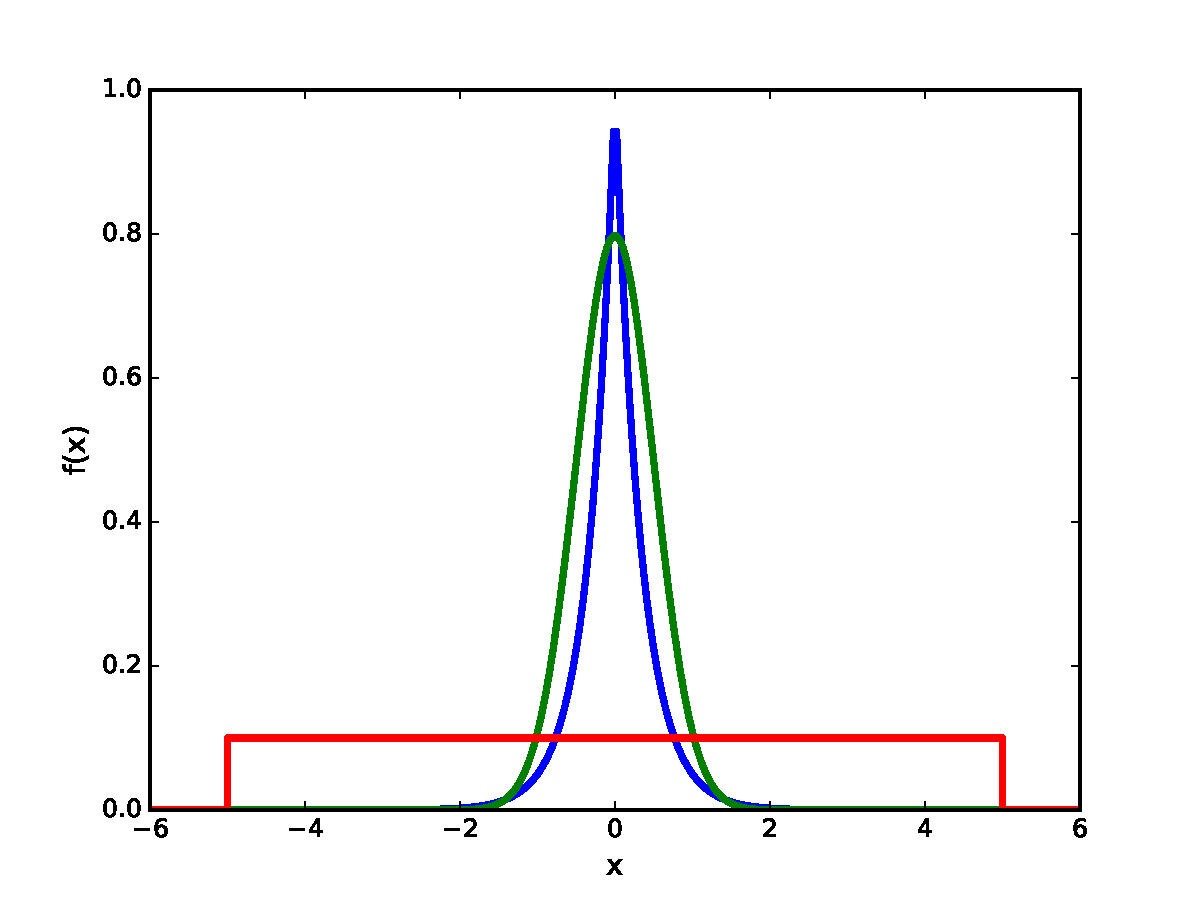
\includegraphics[width=\textwidth]{importanceSampling}
		\caption{A simple importance sampling example (see equation~\ref{eqn:simpleIS}).  The integrand, $f(x)$, is shown in blue,
		the importance sampling distribution is shown in green and, for comparison, the uniform probability density function used
		in the naive case of no importance sampling is also shown (in red).}
		\label{fig:simpleIS}
  	\end{figure}

  	Table~\ref{tab:simpleIS} clearly shows the value of an importance sampling approach convergences to the correct result
  	much faster than when we sample uniformly. Of course this tactic relies on us having some prior knowledge of the behaviour of our
  	integrand in order to select the correct probability density function to use which, in more complicated examples is not always
  	possible\footnote{More novel approaches whereby the sampling distribution is modified to improve convergence as the Monte-Carlo
  	iterations are calculated, such as the \texttt{VEGAS} algorithm,
  	exist but they will not be discussed here.}. A more realistic, and relevant, example of importance sampling comes from the
  	cross-section for the production of a $Z^0$ boson in association with dijets.  The matrix element squared for such a process
  	will have following form upon factoring out the $Z^0$ propagator squared:

  	\begin{equation}
  		|\mathcal{M}_{Z^0+jj}|^2 \sim \left|\frac{1}{p_Z^2 - M_Z + i\Gamma_ZM_Z}\right|^2\times f(\text{QCD, EW})\times g(\text{Kinematic}),
  		\label{eqn:schematicZ}
  	\end{equation}

  	where $p_Z$ is the momentum carried by the $Z^0$ boson, $M_Z$ is its mass, $\Gamma_Z$ is its width and $f(\text{QCD, EW})$ will
  	contain all of the coupling information and $g(\text{Kinematic})$ encodes the remainder of the matrix element.  When using a
  	Monte-Carlo approach to generate events of this kind we can use the schematic of \ref{eqn:schematicZ} to \emph{a priori} select
  	an appropriate probability density function to sample from.  Figure~\ref{fig:breitWigner} shows the squared $Z^0$ propagator.
  	Obvious comparisons with figure~\ref{fig:simpleIS} can be drawn in the sense that were we to generate events with a uniform spread
  	of values for $p_Z^2$ we would end with a very slow rate of convergence by oversampling areas where the integrand is very small and slowly varying.

	\begin{figure}[htp]
		\centering
		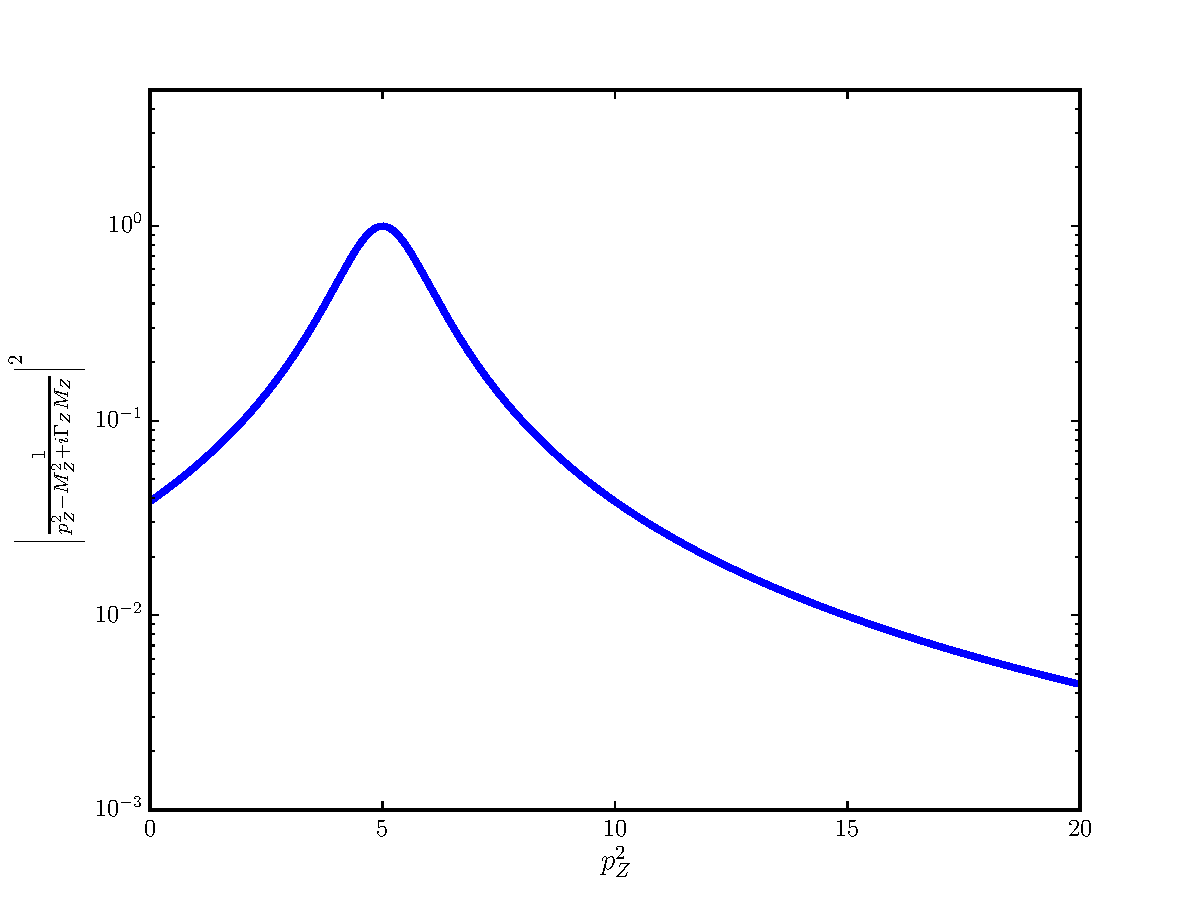
\includegraphics[width=0.8\textwidth, height=0.6\textwidth]{breitWigner}
		\caption{The absolute value squared of the $Z^0$ propagator for a range of values of the invariant mass squared of the
		$Z^0$, $p_Z^2$.  We can see it is strongly peaked at the $Z^0$ mass and, as such, is an ideal candidate for using importance sampling.}
		\label{fig:breitWigner}
  	\end{figure}

	\begin{figure}[htp]
		\centering
		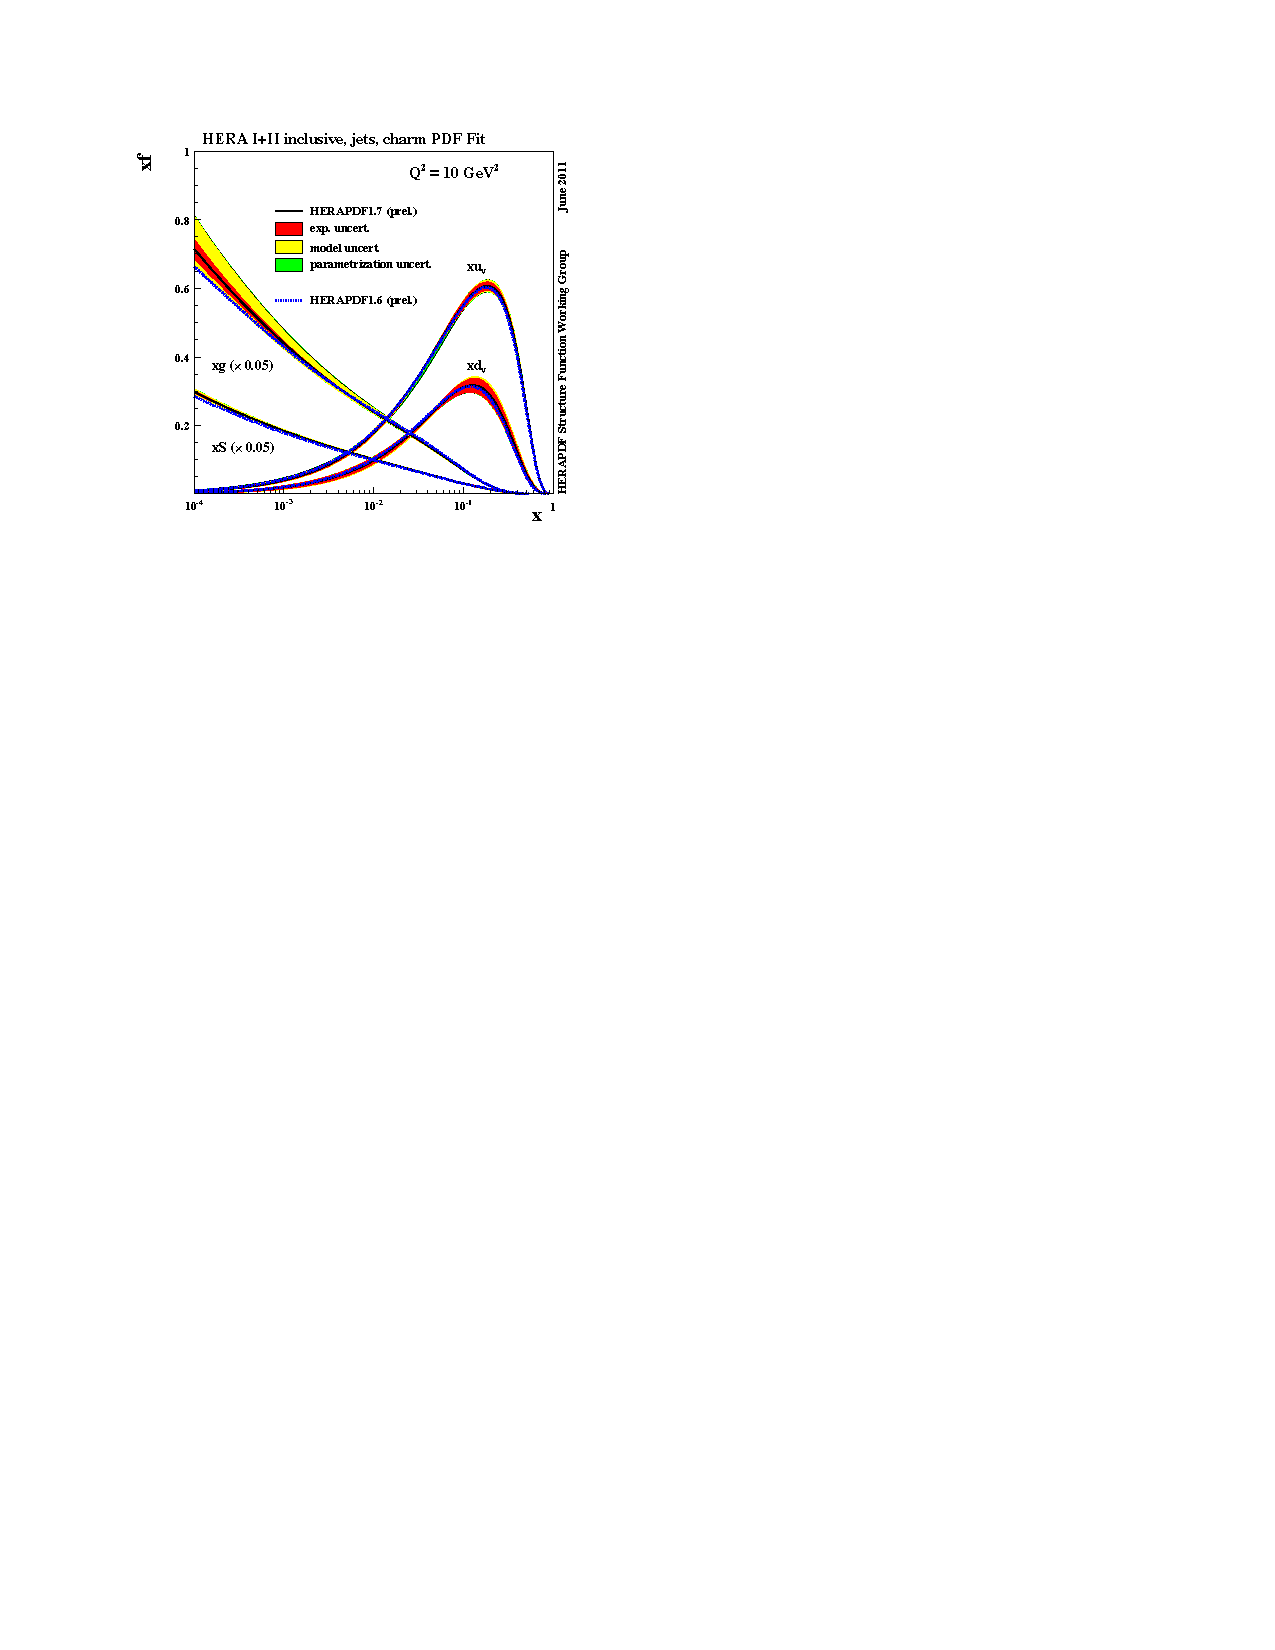
\includegraphics[width=0.8\textwidth, height=0.6\textwidth]{HERAFit}
		\caption{Recent parton distribution function fits from the HERA experiment.  The observed variation in $f(x_{a/b}, Q^2)$, especially at high
		         $x_{a/b}$, can be exploited when computing the equation~\ref{eqn:pdfConvolution} by using an importance sampling approach}
		\label{fig:heraFit}
  	\end{figure}

  	Another good example of importance sampling is found in how we sample the incoming partons in our simulations.  Simple momentum
  	conservation considerations lead us to values for the Bjorken scaling variables of our incoming partons, $x_a$ and $x_b$, and we
  	can use these to intelligently sample the available partons.  The naive way to perform the sum over all possible incoming states
  	would be to uniformly choose a random number corresponding to one of the light quarks, one the light anti-quarks or to a
  	gluon\footnote{By `light (anti-)quarks' we mean all except the top and anti-top.  The parton density functions for these are not available
  	and, even if they were, they would be small enough that we could safely ignore their contribution to cross-sections.}.  We can,
  	however, do better than this by using what we know about how the parton density functions vary with $x_{a/b}$ - figure~\ref{fig:PDFdensities}
  	shows this behaviour as measured by the HERA experiment.  By choosing to randomly sample then incoming parton types according to the relative values
  	for the parton density functions we can, once again, reduce the variance of our numerical integrations as much as possible.

